\documentclass{article}
\usepackage{fullpage}
\usepackage{parskip}
\usepackage{standalone}
\usepackage{graphicx}
\usepackage{booktabs}
\usepackage{subcaption}
\usepackage{hyperref}
\usepackage{xurl}
\usepackage{amsmath}
\usepackage{amsfonts}
\usepackage{amsthm}
\usepackage{empheq}
\usepackage{xfrac}
\usepackage{enumitem}
\usepackage[table]{xcolor}
\usepackage{xfrac}
\usepackage{bbm}
\usepackage{siunitx}
\usepackage{tikz}
\usetikzlibrary{arrows}
\usetikzlibrary{decorations.pathreplacing}
\usetikzlibrary{calc}
\usetikzlibrary{shapes.geometric}
\usetikzlibrary{decorations.markings}
\usetikzlibrary{shapes.geometric}
\usetikzlibrary{patterns,snakes}
\usetikzlibrary{decorations.text}
\usetikzlibrary{arrows.meta}
\usepackage{cases}
\usepackage{tcolorbox}
\usepackage{array}
\usepackage{arydshln}

\setcounter{MaxMatrixCols}{17}

\newtheorem{proposition}{Proposition}


\title{\bf Improving ICU Patient Bed Moves Policies with Reinforcement Learning Based Simulation-Optimisation}
\author{Geraint I. Palmer-Liyu \and Mark Tuson \and Virginia Ahedo \and Paul R. Harper \and Mathew Pugh \and James Williams \and Matt Morgan}

\begin{document}
\maketitle


\section{Introduction}


\section{Background}\label{sec:background}
\begin{tcolorbox}[colback=orange!5!white,colframe=orange!75!black,title=TODO]
Here we need some background on the ICU department at the Heath; background and
literature on on ICU bed moves, why we move patients, why it's bad to move
patients, etc. 
\end{tcolorbox}


\section{ICU Description}\label{sec:description}
The ICU at UHW consists of 35 beds across 4 wards (named A3 North, A3 South, B3
North, and B3 South), two single isolation units, and one double isolation unit.
One bed is generally ring-fenced, left unoccupied, for emergencies.
In each ward there is a partial wall partitioning the beds into two halves.
This is shown in Figure~\ref{fig:icu_map}.
There are two additional units, Complex Care and the Post Anaesthetic Care Unit
(PACU), which generally accommodate their own patient types (complex care and
post anaesthetic patients respectively), spare beds can be used as surge, or
overflow, for general ICU patients when needed.

\begin{figure}
\begin{center}
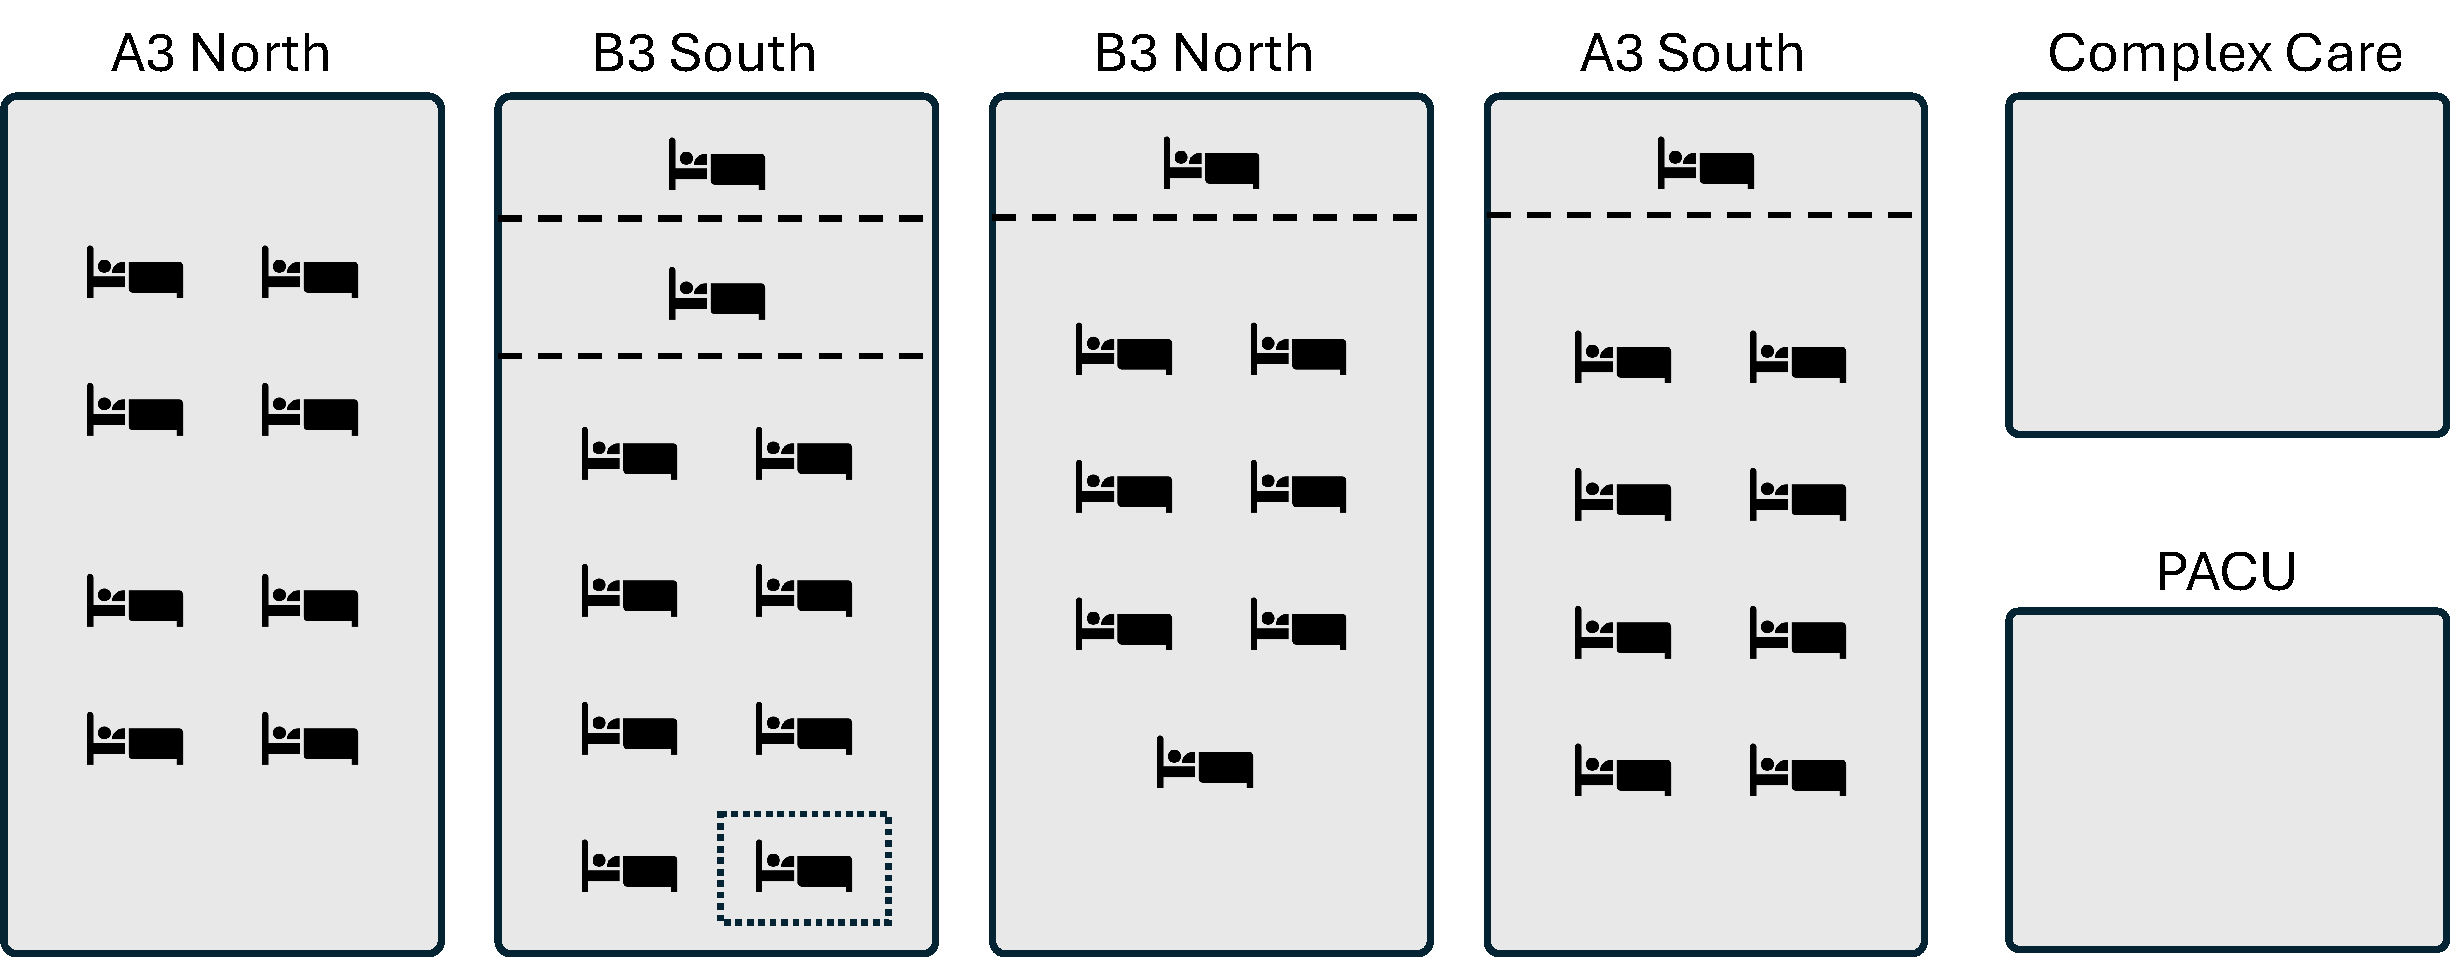
\includegraphics[width=\textwidth]{../images/icu.pdf}
\end{center}
\caption{Representation of the four ICU wards.
Solid blocks represent wards and isolation units, dotted lines represent
partial walls within a ward, and the dotted box represents the ring-fenced bed.}
\label{fig:icu_map}
\end{figure}

The model will consider three types of patient, categorised as Stage 2, Stage 3,
or Stage 3-I patients:
\begin{itemize}
  \item Stage 2: these are the least severe patients.
        When two Stage 2 patients occupy neighbouring beds, both can be cared
        for by the same FTE nurse.
  \item Stage 3: these patients require one to one attention from nurses,
        regardless of patients in neighbouring beds;
  \item Stage 3-I: these patients require isolation and one to one attention.
        When an isolation unit is available, they must be admitted there.
        If an isolation unit is occupied by a Stage 2 or Stage 3 patient, and
        non-isolation bed is available, then the other patient must be moved to
        the available bed and the new Stage 3-I patient must be admitted to the
        isolation unit.
        If they cannot be placed in an isolation unit at all, they are placed in
        a shared unit, and will require their own FTE nurse similar to Stage 3
        patients.
        They will also incur a penalty cost for each time unit they are placed
        in a shared block.
\end{itemize}

In order to make the problem tractable, we make the following simplifications
and assumptions in the model:

\begin{itemize}
  \item the double isolation unit is treated as two separate isolation units.
  The only time this assumption may be violated would be if occupied by a
  patient with a contagious disease, in which case the second bed can then only
  be occupied by a patient with the same contagious disease;
  This is an uncommon enough occurrence to ignore for modelling purposes.
  \item general ICU patients are not admitted to Complex Care or PACU, if there
  are beds available in the other four wards.
  However, Stage 2 patients may be moved there as surge.
  This is generally undesirable, and so incurs some penalty;
  \item a nurse cannot care for two adjacent Stage 2 patients if there is a
  partial wall between the beds;
  \item the ring-fenced bed is never used, it will not be modelled.
\end{itemize}

Data analysis shows that:

\begin{tcolorbox}[colback=orange!5!white,colframe=orange!75!black,title=TODO]
Parametrise these properly, referring back to Section~\ref{sec:background}.
We can do some data analysis here.
\end{tcolorbox}

\begin{itemize}
  \item Stage 2 patients arrive according to the Poisson process with rate $\lambda_0 = 3.0$,
  \item Stage 3 patients arrive according to the Poisson process with rate $\lambda_1 = 2.0$,
  \item Stage 3-I patients arrive according to the Poisson process with rate $\lambda_2 = 1.0$,
  \item Stage 2 patients' lengths of stay are Exponentially distributed with rate $\mu_0 = 0.3$,
  \item Stage 3 patients' lengths of stay are Exponentially distributed with rate $\mu_1 = 0.7$,
  \item Stage 3-I patients' lengths of stay are Exponentially distributed with rate $\mu_2 = 0.4$,
  \item Stage 2 patients deteriorate into Stage 3 patients with rate $\delta_{01}$,
  \item Stage 3 patients deteriorate into Stage 3-I patients with rate $\delta_{12}$,
  \item Stage 3 patients improve into Stage 2 patients with rate $\delta_{10}$,
  \item Stage 3-I patients improve into Stage 3 patients with rate $\delta_{21}$.
\end{itemize}

\section{Problem Decomposition}
The 35 bed ICU problem can be decomposed into two sub-problems by introducing
another assumption.
Ignoring the ring-fenced bed, we can grouping wards A3 North and B3 South, and
wards B3 North and A3 South, into two identical components each containing 17
beds.
We then introduce the assumption that newly arriving patients are sent to the
component with the most free beds.
This corresponds to a \textit{load-balancing} arrival discipline,
a join-shortest-queue discipline that takes into consideration the number of
occupied servers as well as queue length \cite{kingman61, gupta07}, which, due
to Poisson thinning, can be modelled using single queue analysis (SQA) with a
state-dependent arrival rate.
This is shown in Figure~\ref{fig:decomposition}.

The state-dependent arrival rate can be found from a preliminary simulation,
built using Ciw~\cite{palmer19}, and parametrised as above, and observing the
proportion of arrivals that enter each component at each state.
The resulting proportions are given in Figure~\ref{fig:sqa}.
SQA now gives us that the arrival rate for each component, when the component's
occupancy is $x$, is $\lambda_2 p(x)$, $\lambda_3 p(x)$, $\lambda_{3I} p(x)$.

\begin{figure}
\begin{center}
\begin{subfigure}{0.55\textwidth}
\begin{center}
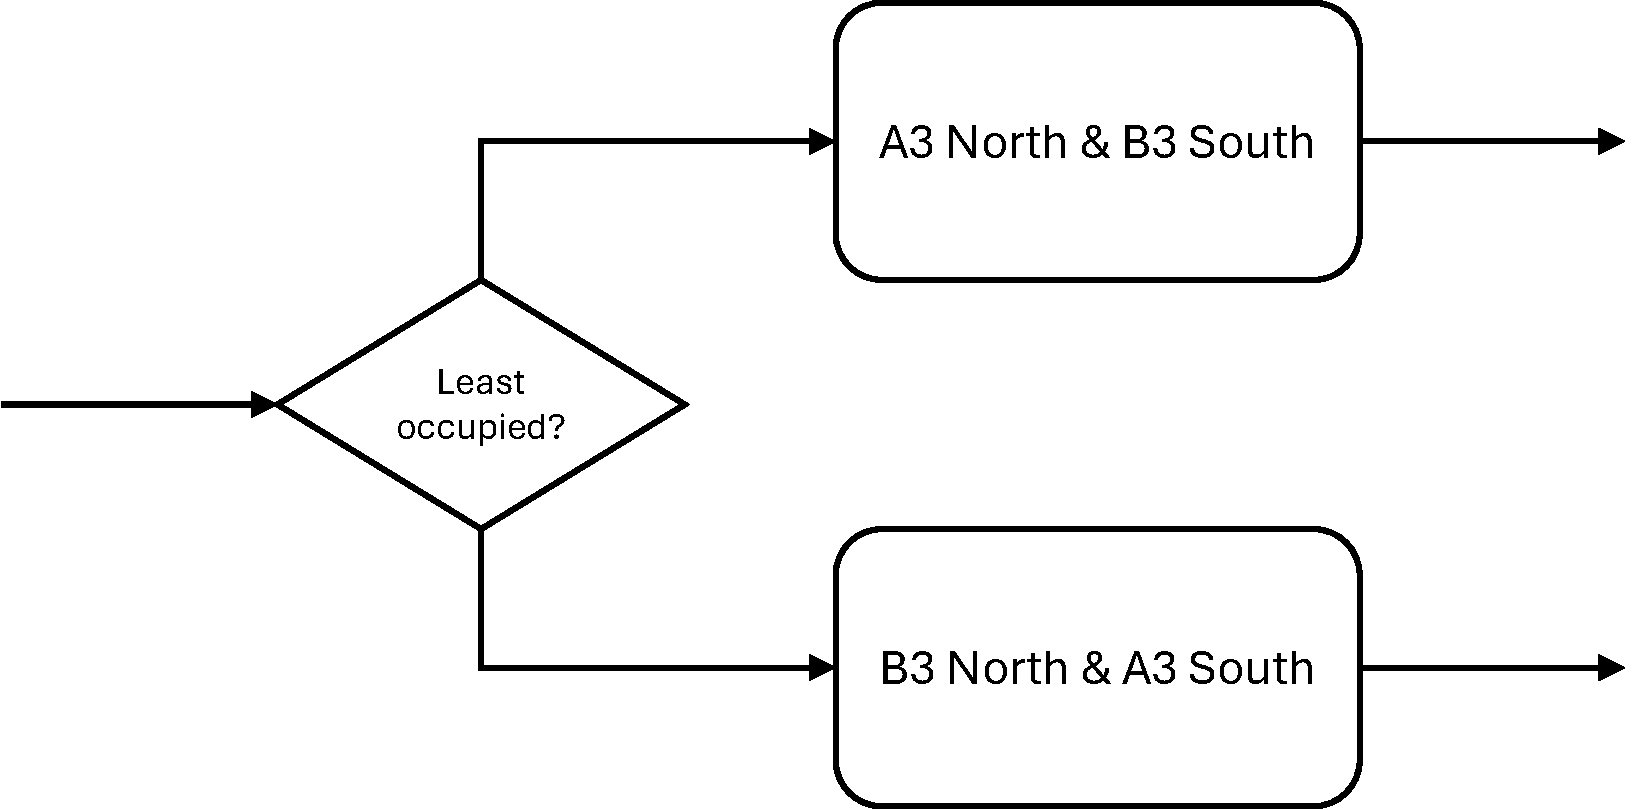
\includegraphics[width=\textwidth]{../images/decomposition.pdf}
\end{center}
\caption{Representation of the load-balancing arrival discipline for the two
identical sub-problems.}
\label{fig:decomposition}
\end{subfigure}
~
\begin{subfigure}{0.35\textwidth}
\begin{center}
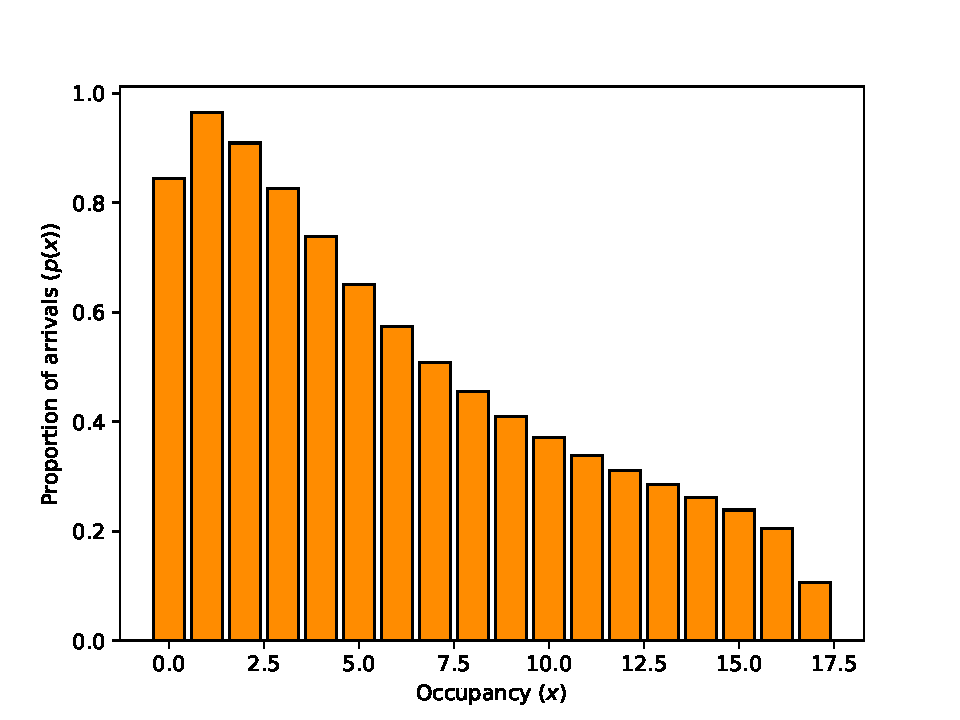
\includegraphics[width=\textwidth]{../plt/sqa.pdf}
\end{center}
\caption{The proportion of the arrivals entering a single component,
given the component's occupancy.}
\label{fig:sqa}
\end{subfigure}
\end{center}
\caption{Problem decomposition analysis}
\label{fig:decomposition_sqa}
\end{figure}

We can now analyse each decomposed sub-problem separately, however each of our
sub-problems are identical, so only one needs to be considered.
The rest of the paper will now consider just one of the decomposed sub-problems,
consisting of an ICU with two wards of 7 and 8 beds, and two isolation units,
giving 17 beds in total. The 8 bed ward is partitioned in two by the partial
wall, while the 7 bed wall is partitioned intro groups of 3 and 4 beds by its
partial wall.


\section{MDP Formulation}
We will consider the bed move policy problem as a Markov Decision Process (MDP),
which is a tuple $(S, A, P, R)$, with states $s \in S$, actions $a \in A$,
transition probabilities $p_{s, s', a} \in P$, and rewards $r_{s, s', a} \in R$.
This is a discrete time MDP, with actions being taken at the discrete events
when a new patient is admitted.
The approach taken to find the optimal policy will be reinforcement learning, a
model-free approach, and so the probabilities $P$ need not be defined, and
transitions are taken care of with a simulation model.
The following sections describe each component.


\subsection{States}\label{sec:states}
The decomposed ICU ward contains 17 beds, which can be partitioned into 4
blocks, shown in Figure~\ref{fig:block_structure}.
These blocks are defined by physical walls: beds B00 to B07 are in one room,
beds B08 to B14 are in another room, and beds B15 and B16 are in isolation
units.
Partial walls do not count as ward separations.
These blocks will determine the cost of a bed-move: intra-block moves are easier
than inter-block moves, and their cost or penalty will reflect this.

\begin{figure}
\begin{center}
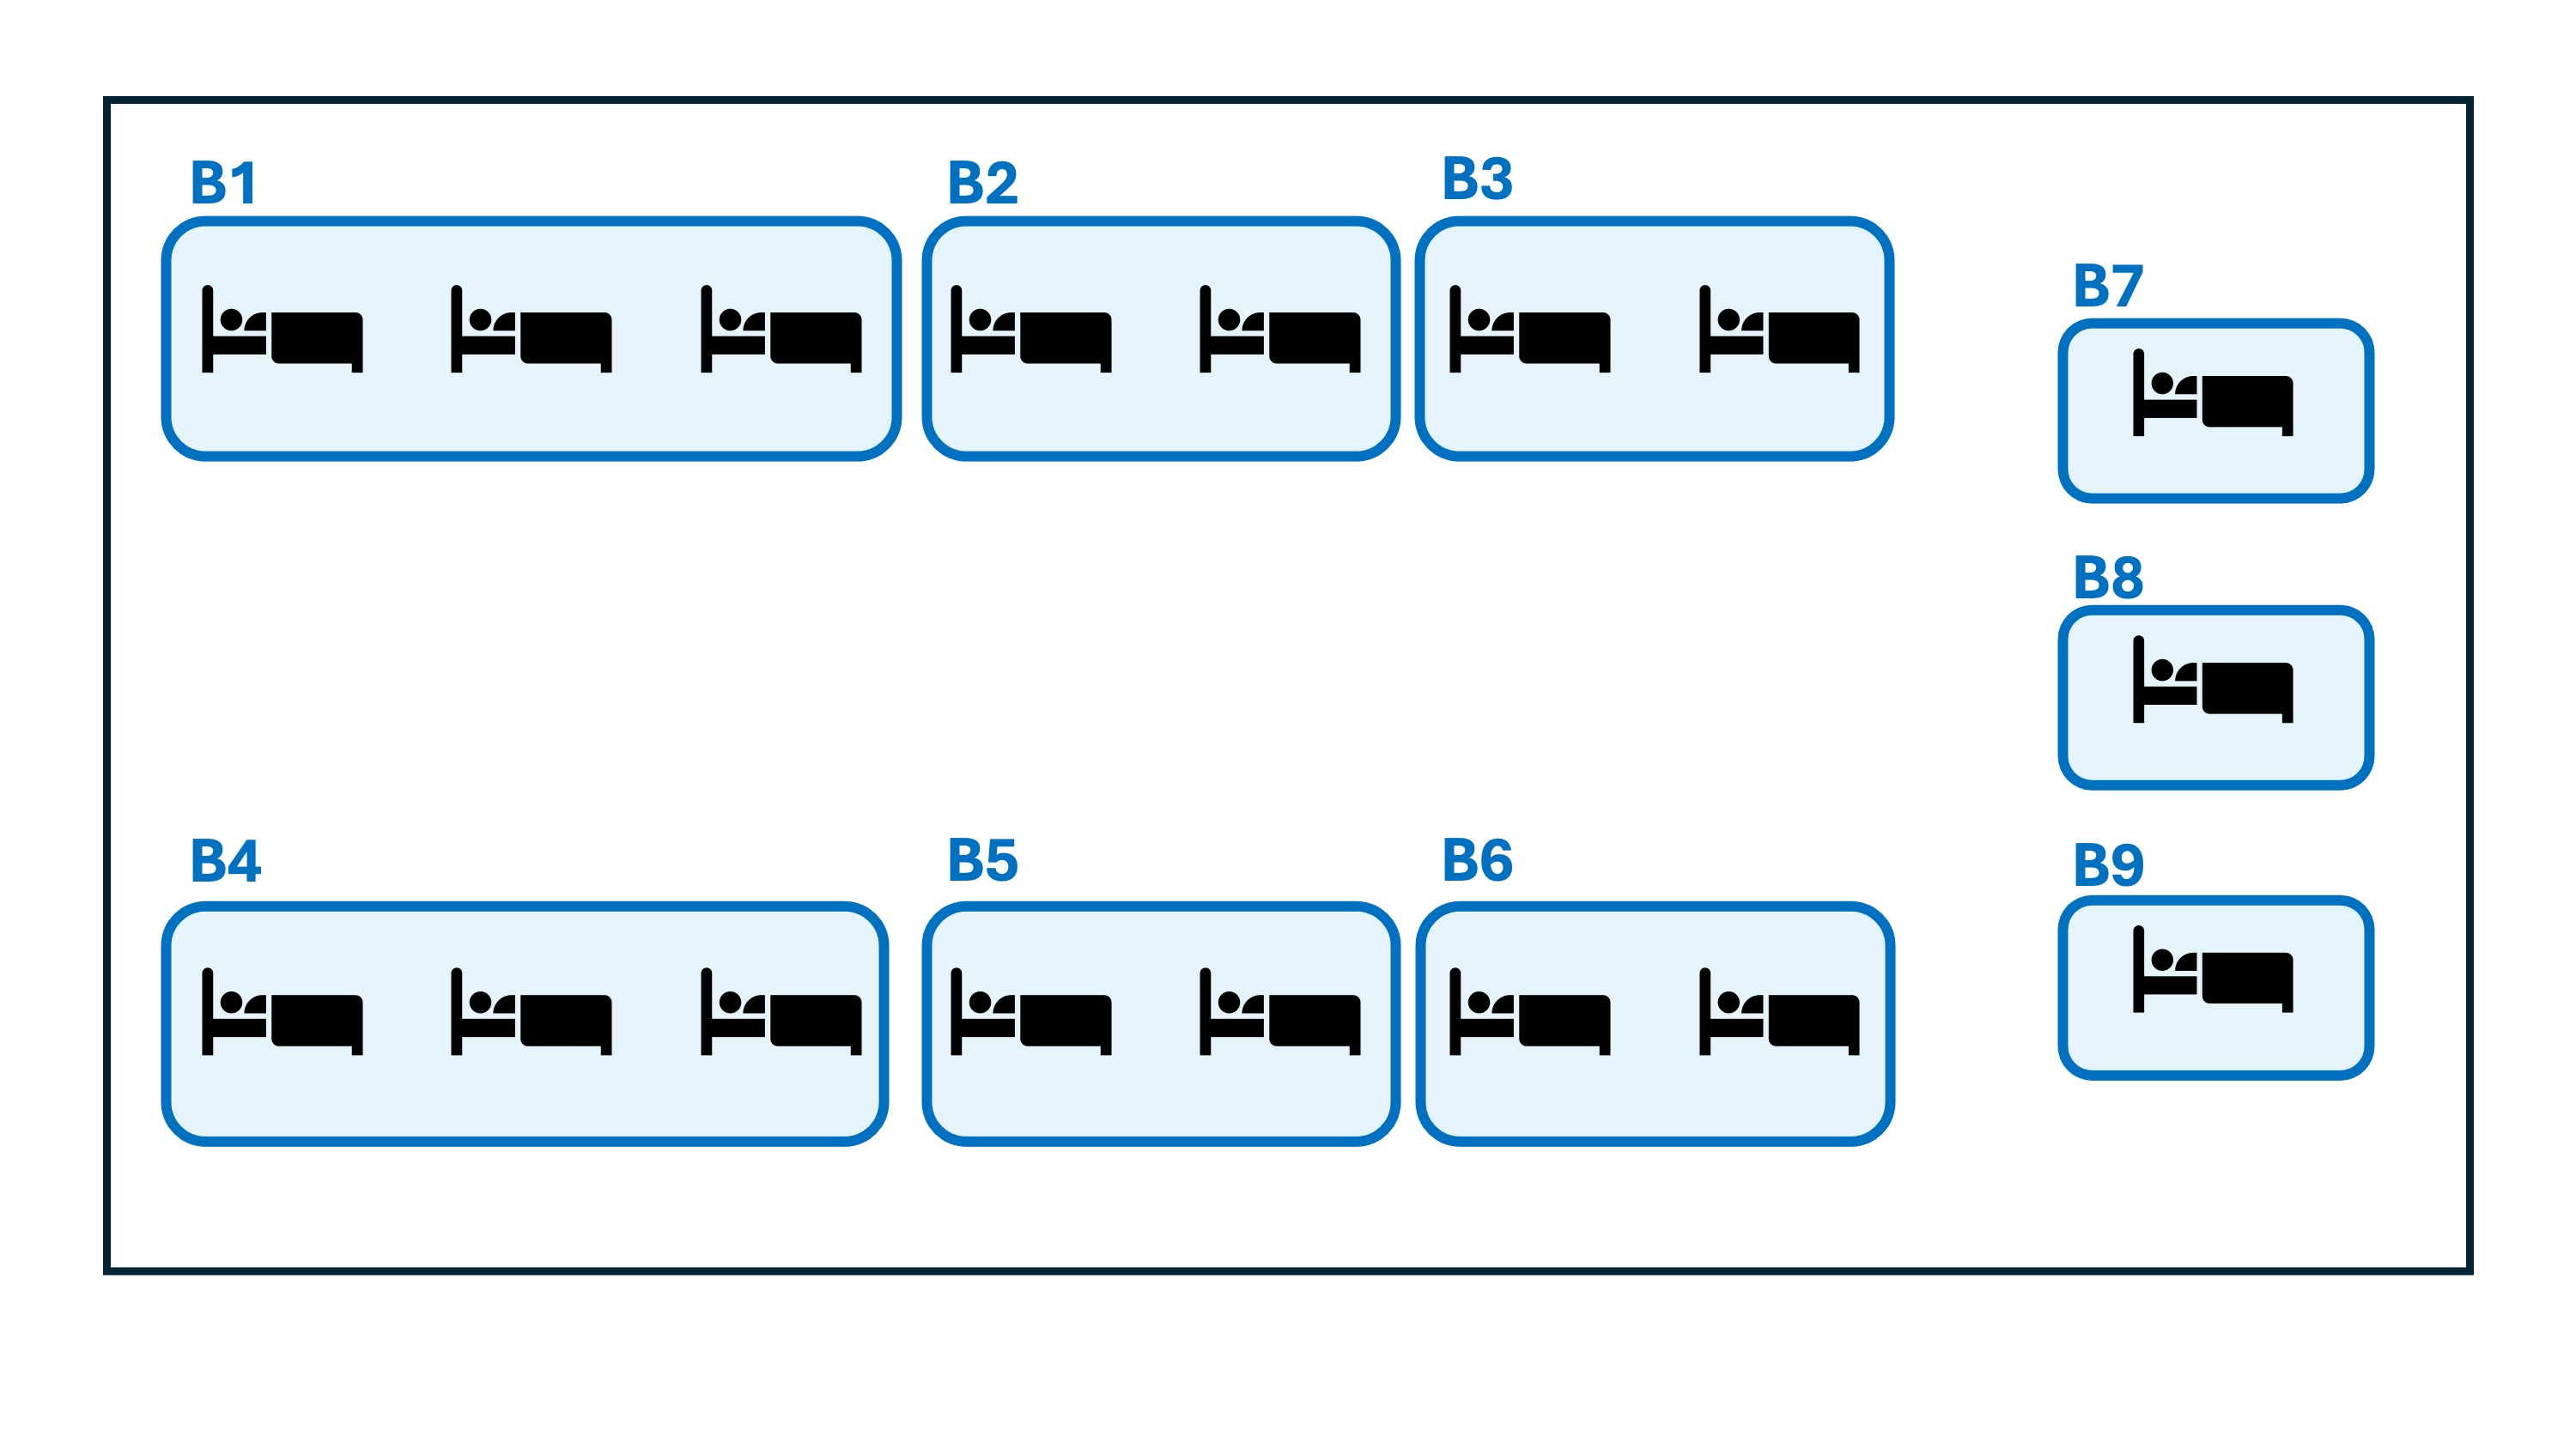
\includegraphics[width=0.7\textwidth]{../images/block_structure}
\end{center}
\caption{Representation of the 17 ICU beds partitioned into 4 blocks.}
\label{fig:block_structure}
\end{figure}

Within a block the location of a patient matters: if two Stage 2 patients are
in adjacent beds, it is possible for one FTE nurse to care for both.
This is shown in Figure~\ref{fig:resource_use}.
Therefore the states need to hold information on both the patient type, and
which particular bed within a block the patient is in.
However, both isolation units are indistinguishable from one another, so there
is no need to differentiate these.

\begin{figure}
\begin{center}
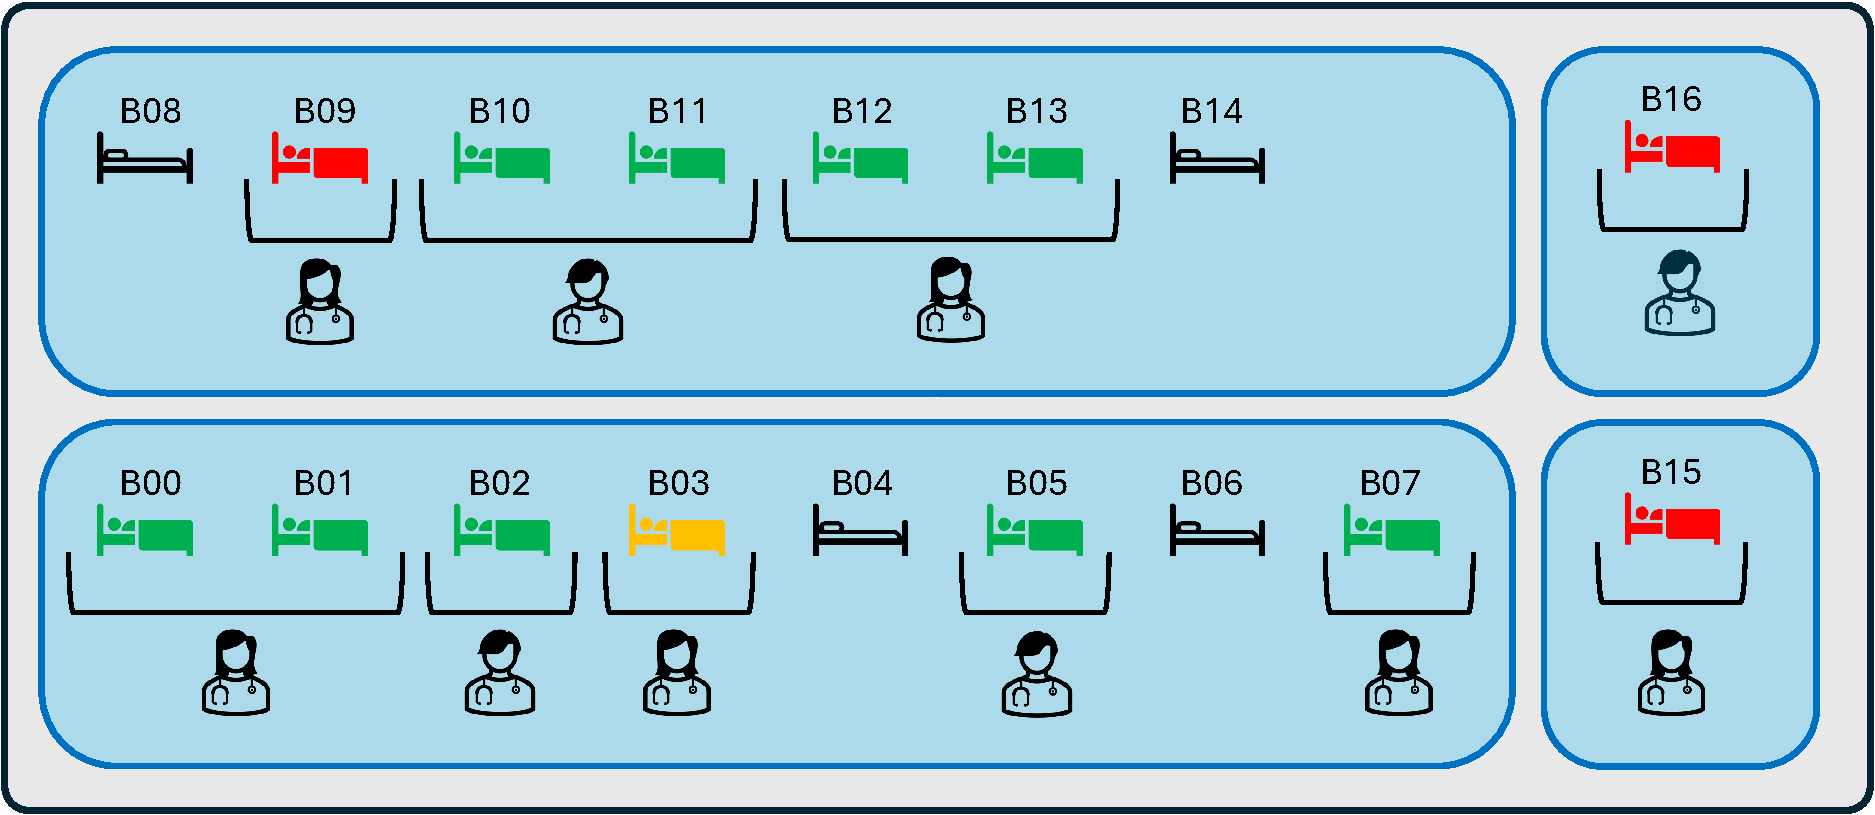
\includegraphics[width=0.7\textwidth]{../images/resource_use}
\end{center}
\caption{Representation of how nurses can share adjacent Stage 2 patients.}
\label{fig:resource_use}
\end{figure}

Define the ward state by a $3\times16$ matrix $M$, where rows correspond to
patient types (where $j=0$ corresponds to Stage 2 patients, $j=1$ to Stage 3
patients, and $j=2$ to Stage 3-I patients), and columns corresponding to bed
numbers (except for column 15, which corresponds to both isolation units).
Then its integer entries $M_{ij}$ denote the number of category $j$ patients
currently occupying a bed $i$.
Note that for columns 0 to 14 the columns sums should be no more than 1, as they
correspond to single beds, while for column 15 the sum should be no more than 2,
as it corresponds to both isolation units.
Let $\mathcal{M}$ denote the set of all possible matrices $M$.

As an example, consider the ICU state given in Figure~\ref{fig:resource_use},
where green, amber and red beds indicate beds occupied by Stage 2, Stage 3 and
Stage 3-I patients respectively, and black beds are unoccupied.
This corresponds to the ward state:

\begin{equation}\label{eqn:example_M}
M^{\star} = \left(\begin{array}{cccc ;{0.6pt/1.4pt} cccc ;{0.6pt/1.4pt} cccc ;{0.6pt/1.4pt} ccc ;{0.6pt/1.4pt} c}
1 & 1 & 1 & 0 & 0 & 1 & 0 & 1 & 0 & 0 & 1 & 1 & 1 & 1 & 0 & 0 \\
0 & 0 & 0 & 1 & 0 & 0 & 0 & 0 & 0 & 0 & 0 & 0 & 0 & 0 & 0 & 0 \\
0 & 0 & 0 & 0 & 0 & 0 & 0 & 0 & 0 & 1 & 0 & 0 & 0 & 0 & 0 & 2
\end{array}\right)
\end{equation}


Ward state changes are caused by newly arriving patients of different categories
being placed into beds in specific blocks, patient discharges, patient
deterioration or improvement (a patient changing type), and moving a patient
from one bed to another.

Actions only take place when a new patient arrives to the ward, and this patient
can be either Stage 2, Stage 3, or Stage 3-I (category $0$, $1$, or $2$).
Therefore the states of the MDP also need to contain information about the newly
arriving patient.
Note that Stage 2 patients cannot arrive when the ward is full, while Stage 3
and Stage 3-I patients can arrive when the ward is full, only if there is a
Stage 2 patient present for them to displace.
Let

\begin{equation*}
s = (M, p)
\end{equation*}

represent the state of the MDP, where $M$ is a $3\times16$ matrix representing
the ward state, and $p \in \{0, 1, 2\}$ indicate the category of the arriving
patient.
Note that we only need states where a patient can arrive.

\begin{proposition}
Let $S$ be the set of all possible states $s = (M, p)$.
Then $|S| = 32,111,460,252$.
\end{proposition}

\begin{proof}
First consider $|\mathcal{M}|$, the number of matrices $M$ that exist.

\begin{itemize}
  \item For each of the first 15 columns representing beds not in an isolation
  unit, $M_{i,j} \in \{0, 1\}$, and the column sum $M_{\cdot, j} \leq 1$.
  There are four ways to satisfy this:

  $$
  \left\{
  \left(\begin{smallmatrix}0\\0\\0\\\end{smallmatrix}\right),
  \left(\begin{smallmatrix}1\\0\\0\\\end{smallmatrix}\right),
  \left(\begin{smallmatrix}0\\1\\0\\\end{smallmatrix}\right),
  \left(\begin{smallmatrix}0\\0\\1\\\end{smallmatrix}\right)
  \right\}
  $$

  Each column is independent of the rest, and so there are $4^{15}$
  configurations for these columns.

  \item For the final column, representing the isolation units,
  $M_{i,15} \in \{0, 1, 2\}$, and the column sum $M_{\cdot, 15} \leq 2$.
  There are ten ways to satisfy this:

  $$
  \left\{
  \left(\begin{smallmatrix}0\\0\\0\\\end{smallmatrix}\right),
  \left(\begin{smallmatrix}1\\0\\0\\\end{smallmatrix}\right),
  \left(\begin{smallmatrix}1\\1\\0\\\end{smallmatrix}\right),
  \left(\begin{smallmatrix}1\\0\\1\\\end{smallmatrix}\right),
  \left(\begin{smallmatrix}0\\1\\0\\\end{smallmatrix}\right),
  \left(\begin{smallmatrix}0\\1\\1\\\end{smallmatrix}\right),
  \left(\begin{smallmatrix}0\\0\\1\\\end{smallmatrix}\right),
  \left(\begin{smallmatrix}2\\0\\0\\\end{smallmatrix}\right),
  \left(\begin{smallmatrix}0\\2\\0\\\end{smallmatrix}\right),
  \left(\begin{smallmatrix}0\\0\\2\\\end{smallmatrix}\right)
  \right\}
  $$

  This column is independent of the others, and so there are $10 \times 4^{15}$
  possible matrices $M$ representing valid system states.
\end{itemize}

However, not all states admit an arriving patient:

\begin{itemize}
  \item Stage 2 patients cannot arrive if the ward is full.
  There are 3 ways in which each of the first 15 columns can be full, and 6 ways
  the final column can be full, and so there are $6 \times 3^{15}$ that can be
  discarded for when $p = 0$.

  \item Stage 3 and 3-I patients can arrive if the system is full, as long as
  there is a Stage 2 patient present to displace and send to surge.
  There are 2 ways in which each of the first 15 columns can be full without a
  Stage 2 patient, and 3 ways for the final column, therefore there are
  $3 \times 2^{15}$ states that can be discarded when $p \in \{1, 2\}$.
\end{itemize}

Therefore the total number of states $s = (M, p)$ is:

\begin{align*}
|S| &= (3 \times 10 \times 4^{15}) - (2 \times 3 \times 2^{15}) - (6 \times 3^{15})\\
&= 32,111,460,252
\end{align*}

\end{proof}


\subsubsection{State Equivalences}\label{sec:state_equivalences}

The state matrices exhibit some equivalences.
In the three blocks of 4, and the block of 3, reversed configurations are
equivalent up to a bed labelling.
This is shown in Figure~\ref{fig:symmetries}.
Similarly, as the two blocks of 4 beds that are located in the same ward are
identical, then swapping the configurations result in equivalent
configurations up to a labelling.

\begin{figure}
\begin{center}
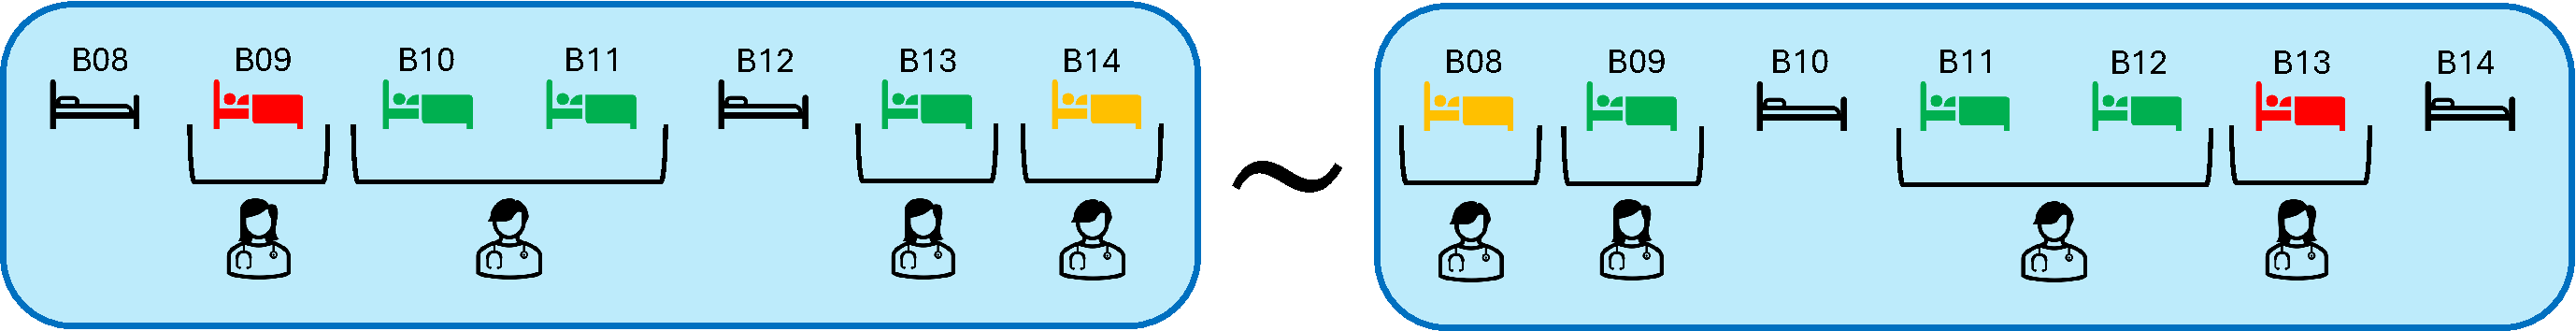
\includegraphics[width=0.7\textwidth]{../images/symmetries.pdf}
\end{center}
\caption{Example of an equivalence in a block of 4 beds.}
\label{fig:symmetries}
\end{figure}

Therefore define four column-transformation operations on $\mathcal{M}$
corresponding to these equivalences:
\begin{itemize}
  \item $T_1$: reversing columns 0 to 3;
  \item $T_2$: reversing columns 4 to 7;
  \item $T_3$: reversing columns 8 to 11;
  \item $T_4$: reversing columns 12 to 14;
  \item $T_5$: swapping the block of columns 0–3 with the block 4–7.
\end{itemize}

We will consider all combinations of compositions of these transforms, and it
will be useful later to understand their inverses.
Note that all five of these transforms are involutions, that is they are their
own inverse, and applying the same transform twice will give the original
matrix.
As the first four concern non-overlapping columns, then they are commutative
under composition, and so any combination of these, $P$ is also an involution
\cite[p.~22]{dummit04}, and $P^{-1} = P$.
This is not true however composing $T_5$ and $T_1$ or $T_2$ as they affect the
same columns.
However, if we $T_5$ was applied first or last, that is
$P = \tilde{T} \circ T_5$ or $Q = T_5 \circ \tilde{T}$ where $\tilde{T}$ is some
combination of the other transforms, then we can use that permutation as the
inverse if we apply and re-apply $T_5$:

\begin{align}
T_5 \circ P \circ T_5
&= T_5 \circ (\tilde{T} \circ T_5) \circ T_5
= T_5 \circ \tilde{T} \circ I
= T_5 \circ \tilde{T}
= T_5^{-1} \circ \tilde{T}^{-1}
= P^{-1}, \;\; \text{or} \\
T_5 \circ Q \circ T_5
&= T_5 \circ (T_5 \circ \tilde{T}) \circ T_5
= I \circ \tilde{T} \circ T_5
= \tilde{T} \circ T_5
=  \tilde{T}^{-1} \circ T_5^{-1}
= Q^{-1}
\end{align}

which are the exact inverse of $P$ and $Q$ \cite[p.~18]{dummit04}.

Now define a relation $\sim$ on $\mathcal{M}$ such that $M_1 \sim M_2$ if $M_2$
is obtained by applying some sequence of the column-transformations above on
$M_1$.
It is clear that $\sim$ satisfies reflexivity, symmetry, and transitivity, and
is therefore an equivalence relation, and so $\mathcal{M}$ can be partitioned
into disjoint equivalence classes
$[M_1] = \{M_2 \in \mathcal{M} \mid M_2 \sim M_1\}$.
Now define $\mathcal{M}^{\star} \subseteq \mathcal{M}$ to be the set containing
exactly one representative matrix from each equivalence class.
How this representative matrix is chosen is detailed in
Section~\ref{sec:representative}.
Hence, we can also define $S^{\star}$ as the set of all possible states
$s = (M, p)$ where $M \in \mathcal{M}^{\star}$, that is the set of all
representative states.

\begin{proposition}\label{thrm:generate_equivalence_classes}
A list of all elements of an equivalence class $[M]$ can be generated by
applying all combinations of the transformations in
$\{T_1, T_2, T_3, T_4, T_5\}$ to $M$, where the transforms in each composition
are ordered by strictly increasing indices.
\end{proposition}

This means, for example, that $T_1 \circ T_3 \circ T_4$ is evaluated, while an
alternative ordering like $T_3 \circ T_1 \circ T_2$ is excluded.
$T_1 \circ T_4 \circ T_1 \circ T_2$ is also excluded as we do not repeat
transformations.

\begin{proof}
By definition $[M]$ contains all elements that can be reached from $M$ by
applying any combination of transforms in $\{T_1, T_2, T_3, T_4, T_5\}$,
including repeats, in any order.


\begin{itemize}
  \item First consider a permutation $P$ that does not use $T_5$, the block-swap
  transformation.
  As all other transforms commute, we can apply the transforms in any order
  without changing $P$, and so we can obtain $P$ by applying the transforms by
  strictly increasing indices.
  As for repeated application of any of the transforms, as they are involutions,
  any two consecutive repeated applications of the same transform cancel out, so
  $P$ needs at most one application of each transform.
  Therefore $P$ will be found by the generation scheme.

  \item Now consider a permutation $Q$ that does contain at least one
  application of $T_5$.

  The only transforms that do not commute with $T_5$ are $T_1$ and $T_2$ as they
  operate on the same columns.
  Notice that:

  \begin{align*}
  T_5 \circ T_1 &= T_2 \circ T_5 \\
  T_5 \circ T_2 &= T_1 \circ T_5
  \end{align*}

  From this it is always possible to re-write $Q$ as a composition of transforms
  where all $T_5$ transforms are always applied either first or last; and the
  sequence of applications $T_5$ can be reduce to either one or no applications
  of $T_5$ as this is an involution.
  The remaining of the sequence of transforms can be treated as $P$, which can
  be written as a sequence of unique transforms by strictly increasing indices.
  Therefore $Q$ will be found by the generation scheme.
\end{itemize}
\end{proof}

As there are five equivalences, $|[M]| \leq 2^5 = 32$. By generating all 32 permutation using Proposition~\ref{thrm:generate_equivalence_classes} we ensure
all equivalent states are found, though some may duplicate.
We can generate these in order in such a way that the first 16 elements do not
use $T_5$ while the second 16 do use $T_5$, implying that knowing if our
permutation is in the first of second half of our list, we know which inverse
scheme to use: $P$ if it is in the first half, and $T_5 \circ P \circ T_5$ if it
is in the second half of the list.


\begin{tcolorbox}[colback=orange!5!white,colframe=orange!75!black,title=TODO]
Enumerate combinatorially how many valid representative MDP states exist.
Due to the five equivalences, I expect this to be around $2^5 = 32$ times smaller,
not including symmetric states.
\end{tcolorbox}


\subsection{Actions}\label{sec:actions}
Define an action as an operator on an MDP state $s \in S$ to a ward state
$M \in \mathcal{M}$.
An action is placing a newly arriving patient into a bed, either unoccupied or
occupied.
If placing into an occupied bed, then the patient currently occupying that bed
needs to be moved either into an unoccupied bed or into surge.
We can denote an action by a pair of integers $(b, d)$.
When $b = d$ this denotes placing the newly arriving patient into bed $b$ where
that bed is unoccupied.
When $b \neq d$ this denotes placing the newly arriving patient into bed $b$,
and moving patient occupying bed $b$ to bed $d$.
When $d = 16$ this denotes moving the patient to surge.

For example, action $a = (3, 6)$ represents placing a patient into bed 3, and
moving the patient currently in bed 3 to bed 6, e.g.:

\begin{equation}\label{eqn:example_action}
a(M^{\star}, 2) = \left(\begin{array}{cccc ;{0.6pt/1.4pt} cccc ;{0.6pt/1.4pt} cccc ;{0.6pt/1.4pt} ccc ;{0.6pt/1.4pt} c}
1 & 1 & 1 & 0 & 0 & 1 & 0 & 1 & 0 & 0 & 1 & 1 & 1 & 1 & 0 & 0 \\
0 & 0 & 0 & 0 & 0 & 0 & 1 & 0 & 0 & 0 & 0 & 0 & 0 & 0 & 0 & 0 \\
0 & 0 & 0 & 1 & 0 & 0 & 0 & 0 & 0 & 1 & 0 & 0 & 0 & 0 & 0 & 2
\end{array}\right)
\end{equation}

where $M^{\star}$ is the ward state defined in Equation~\ref{eqn:example_M}.

Actions are state-dependent:
\begin{itemize}
  \item only Stage 2 patients can be moved into surge;
  \item arriving Stage 3-I patients \textit{must} be placed into an isolation
  unit if free, or they \textit{must} move Stage 2 or Stage 3 patients out of an
  isolation unit if no isolation unit is free. When there is a choice of patient
  type to move out of an isolation unit, Stage 2 patients are moved.
\end{itemize}

The set of actions available when in a particular state $s = (M, p)$, denoted by
$A_s$, will depend on the ward state component, $M$ and the arriving patient
type $p$, such that the constraints above hold.
That is:

\begin{equation}
A_s = \{ (b, d) \mid b \in \{0, \dots, 15\}, \, d \in \{0, \dots, 16\} \}
\end{equation}

Subject to:

\begin{empheq}[left=\empheqlbrace]{align}
    b=d &\implies M_{\cdot,b}=0 \label{eqn:action_1}\\
    b \neq d \text{ and } d < 16 &\implies M_{\cdot, d} < K_d \text{ and } M_{\cdot, b} > 0 \text{ and } M_{p,b} = 0 \label{eqn:action_2}\\
    d=16 &\implies p \neq 0 \text{ and } M_{0,b} > 0 \label{eqn:action_3}\\
    p=2 \text{ and } M_{\cdot, 15} < 2 &\implies b=d=15 \label{eqn:action_4}\\
    p=2 \text{ and } M_{\cdot, 15} = 2 \text{ and } M_{2, 15} \neq 2 &\implies b=15 \text{ and } (M_{\cdot, d} = 0 \text{ or } d=16) \label{eqn:action_5}\\
    p=2 \text{ and } M_{\cdot, 15} = 2 \text{ and } M_{2, 15} = 2 &\implies b \neq 15 \text{ and } (M_{\cdot, d} = 0 \text{ or } d=16) \label{eqn:action_6}
\end{empheq}

where $K_j = 1$ for all $j < 15$, and $K_{15} = 2$.
Constraint~\ref{eqn:action_1} corresponds to placing a newly arriving patient in
an empty bed without any bed moves; constraint~\ref{eqn:action_2} corresponds to
placing the newly arriving patient into bed $b$, moving the current occupier to
bed $d$; constraint~\ref{eqn:action_3} corresponds to only being able to move a
Stage 2 patient to surge; constraint~\ref{eqn:action_4} corresponds to needing
to place a newly arriving Stage 3-I patient into a free isolation unit; and
constraint~\ref{eqn:action_5} corresponds to needing to move a less severe
patient from an isolation unit to make room for an arriving Stage 3-I patient,
and constraint~\ref{eqn:action_6} allows placing a Stage 3-I patient in another
bed only if the isolation units are full with other Stage 3-I patients.
Note that constraints~\ref{eqn:action_2} and~\ref{eqn:action_3} also restrict
displacing a patients of the same type, as this would result in an equivalent
state to placing them directly in an empty bed.

\begin{tcolorbox}[colback=orange!5!white,colframe=orange!75!black,title=TODO]
Enumerate combinatorially how many valid MDP states-action pairs exist.
\end{tcolorbox}

These action sets are defined for all states $s \in S$, however due to state
equivalences, we only need to define them for all $s \in S^{\star}$.
When in state $s \neq S^{\star}$, we transform $s$ my permutation $P$ into a
representative of its equivalence class, such that $P(s) \in S^{\star}$,
These state equivalences mean that when the simulation visits a particular
state-action pair, the reinforcement learning agent will update the $Q$-value
of a representative state-action pair.
This is given in Proposition~\ref{thrm:representative_stateaction}, where
applying the permutation to a state corresponds to applying the permutation to
the corresponding ward state matrix: $P(s) = (P(M), p)$.

\begin{proposition}\label{thrm:representative_stateaction}
For the state-action pair $(s, a)$, the representative state-action pair is
$(P(s), P^{-1}(a))$, where $P$ is the permutation that takes the state to its
representative state.
\end{proposition}

\begin{proof}
Let $s$, $a$ and $P$ be given, such that $P$ is the permutation that takes
state $s$ to its representative state.
Let $(s', a')$ be the representative state-action pair.

It is clear that the state component of the representative state-action pair,
$s' = P(s)$, be definition of $P$.

If applying $a(s) = \tilde{s}$, we wish to find an action $a'$ such that
$a'(s') = \tilde{s}'$, and that $\tilde{s}'$ can be reached from $\tilde{s}$ by
the same permutation $P$.
That is:

\begin{align}
P(\tilde{s}) &= \tilde{s}' \\
P(a(s)) &= a'(s') \\
P(a(s)) &= a'(P(s))
\end{align}

We wish that this relationship be true for any state $s$, and so we want the
operations $P \circ a$ and $a' \circ P$ are equal:

\begin{align}
a' \circ P &= P \circ a \\
a' \circ P \circ P^{-1} &= P \circ a \circ P^{-1} \\
a' \circ \mathbb{I} &= P \circ a \circ P^{-1} \\
a' &= P \circ a \circ P^{-1} \label{eqn:conjugate}
\end{align}

where Equation~\ref{eqn:conjugate} is a conjugation, which on permutations
acts as a relabelling, we have that $a' = P^{-1}(a)$ \cite[p.~125]{dummit04},
hence $(s', a') = (P(s), P^{-1}(a))$ as required.
\end{proof}


\subsubsection{Action Equivalences}\label{sec:action_equivalences}

If two actions transform a state two different yet equivalent matrices, we only
need to consider one of these actions.
For example consider actions $a_1 = (8, 12)$, $a_2 = (8, 14)$, $a_3 = (11, 12)$,
and $a_4 = (11, 14)$ operating on a state $s = (M, 2)$, where
Figure~\ref{fig:action_symmetries} shows beds B08 to B14 of $M$, before and
after applying these actions - the resulting states are equivalent due to
transforms $T_3$, $T_4$ and $T_3 \circ T_4$.

\begin{figure}
\begin{center}
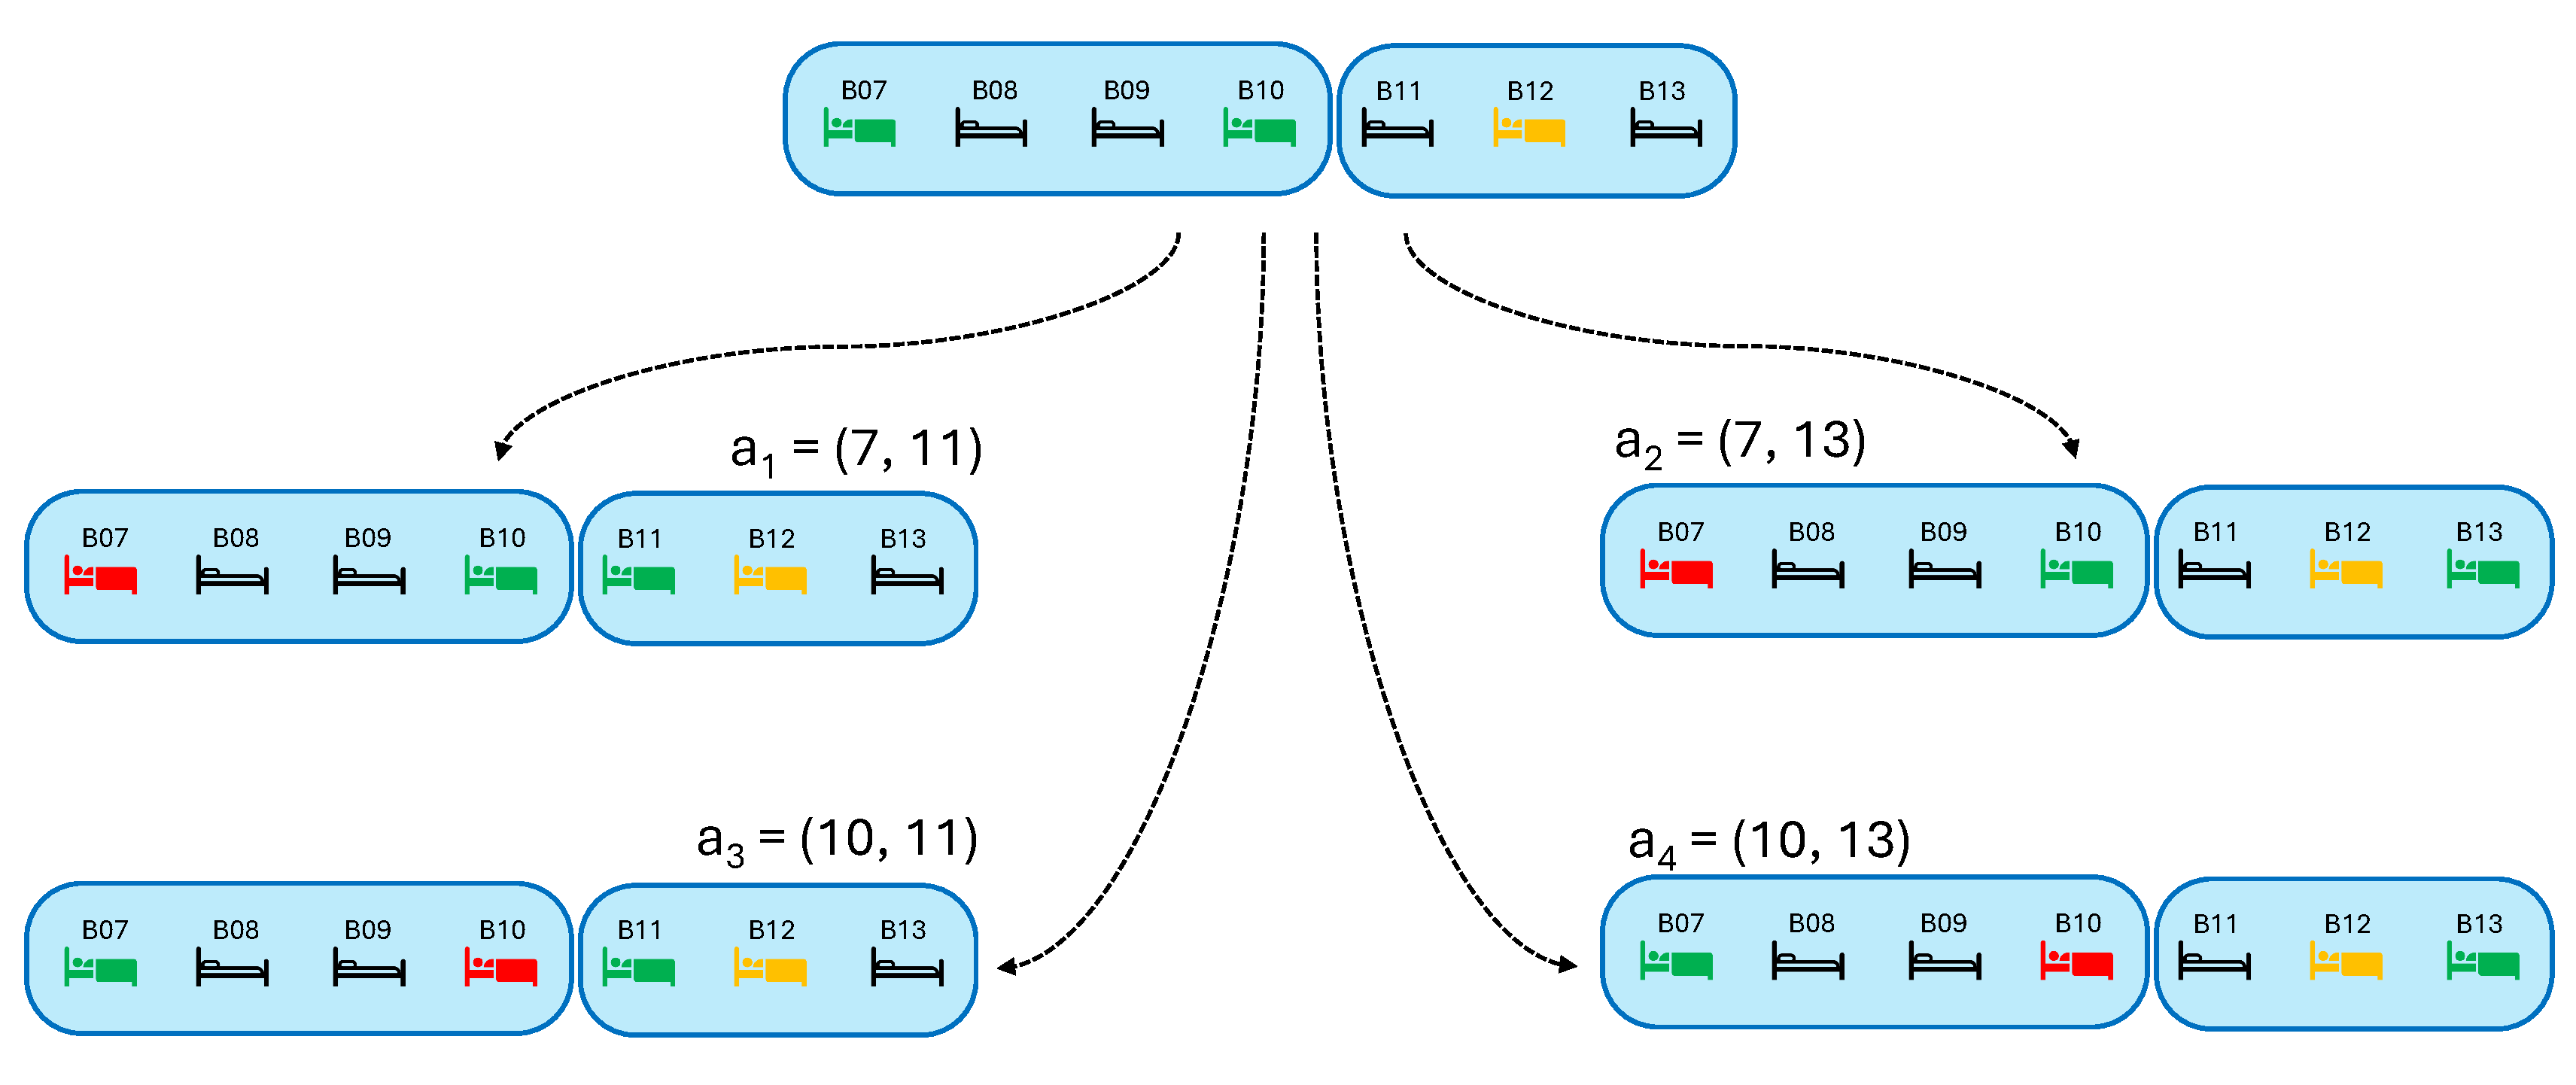
\includegraphics[width=\textwidth]{../images/action_symmetries.pdf}
\end{center}
\caption{Example of an action equivalence.}
\label{fig:action_symmetries}
\end{figure}

Therefore define a relation $\equiv$ such that
$a_1 \equiv a_2$ if $a_2(s) \sim a_1(s)$, that is if the ward states they
produce belong to the same equivalence class.
It is clear that $\equiv$ also satisfies reflexivity, symmetry, and
transitivity, and so is also an equivalence relation.
Hence each set $A_s$ can be partitioned into disjoint equivalence classes
$[a_1] = \{a_2 \in A_s \mid a_2 \equiv a_1\}$, and so we can define
$A_s^{\star} \subseteq A_s$ to be the set containing exactly one representative
action from each equivalence class.
How this representative action is chosen is detailed in
Section~\ref{sec:representative}.

\begin{proposition}
For a state $s = (M,p)$, $A_s$ can contain two equivalent actions when acting on
$s$ if and only if $M$ is a fixed point of some permutation $P$, that is
$P(M) = M$. Under this condition, any action $a = (b,d)$ where either $b$ or $d$
is affected by $P$ has an equivalent action $a' = (P^{-1}(b), P^{-1}(d))$.
\end{proposition}

As a preliminary to the proof, consider that applying an action to a state
results in a matrix that is the sum of the original matrix plus some sparse
difference matrix with elements in $\{-1, 0, 1\}$; consider the example matrix
$M^{\star}$ with $a = (3, 6)$, we have $a(M^{\star}, 2) = M^{\star} + \delta_a$,
where the matrix $\delta_a$ corresponds to removing a Stage 2 patient from bed
B03, inserting a Stage 2 patient into bed B06, and inserting a Stage 3-I
patient into bed B03:

\begin{equation}
\delta_a  =\left(\begin{array}{cccc ;{0.6pt/1.4pt} cccc ;{0.6pt/1.4pt} cccc ;{0.6pt/1.4pt} ccc ;{0.6pt/1.4pt} c}
0 & 0 & 0 & -1 & 0 & 0 & 1 & 0 & 0 & 0 & 0 & 0 & 0 & 0 & 0 & 0 \\
0 & 0 & 0 & 0 & 0 & 0 & 0 & 0 & 0 & 0 & 0 & 0 & 0 & 0 & 0 & 0 \\
0 & 0 & 0 & 1 & 0 & 0 & 0 & 0 & 0 & 0 & 0 & 0 & 0 & 0 & 0 & 0
\end{array}\right)
\end{equation}

Note that if $M$ is a fixed point of multiple permutations,
$P_1, P_2, \dots P_n$, then $a, P_1(a), P_2(a), \dots P_n(a)$ are all
equivalent, though not necessarily unique.  

\begin{proof}
Two actions, $a$ and $a'$ are equivalent if, for some permutation $P$:
\begin{align}
a(M) &= P(a'(M)) \\
M + \delta_a &= P(M + \delta_{a'}) \\
M + \delta_a &= P(M) + P(\delta_{a'}) \label{eqn:linear_permutations}\\
M - P(M) &= P(\delta_{a'}) - \delta_a \label{eqn:action_symmetry_identity}
\end{align}

where Equation~\ref{eqn:linear_permutations} is possible due to column
permutations being linear transforms.
For this to be true:
\begin{itemize}
  \item either $P(M) = M$, and so $M$ is a fixed point of $P$, and
  $P(\delta_{a'}) = \delta_a$, implying that $P(a') = a$, and so
  $a' = P^{-1}(a)$;
  \item or $P(M) \neq M$. In this case the left hand side of
  Equation~\ref{eqn:action_symmetry_identity} must have the property that
  permuted columns have opposite signs.
  For the same property to occur in the right hand side, we must have
  $a' = P(a)$, but this would imply that both sides of the equation are equal
  to zero, hence $P(M) = M$, which is a contradiction.
\end{itemize}

Hence equivalent actions can only arise under permutations $P$ for which $M$ 
is a fixed point, and $a = (b, d) \equiv a' = (P^{-1}(b), P^{-1}(d))$.
In order for $a \neq a'$, then either $b$ or $d$ must be columns affected
by $P$.
\end{proof}

An efficient way is needed to check which of the 32 permutations a state is a
fixed point of.
We propose to do this with a maximum of six checks: because $T_3$ and $T_4$
operate on distinct sets of columns to the other transforms, then a fixed point
of a permutation $P$ that is made up from composing $T_3$ or $T_4$ with any
other combination of transforms must also be a fixed point of $T_3$ or $T_4$
respectively.
The other three transforms interact with the overlapping columns, and so a
decision tree with a maximum of four checks is constructed, shown in
Figure~\ref{fig:fixed_point_decision_tree}.
Hence we can find the full set of permutations that a state is a fixed point of
by checking it is a fixed point of $T_3$, of $T_4$, and then between two and
four checks by following the decision tree.

\begin{figure}
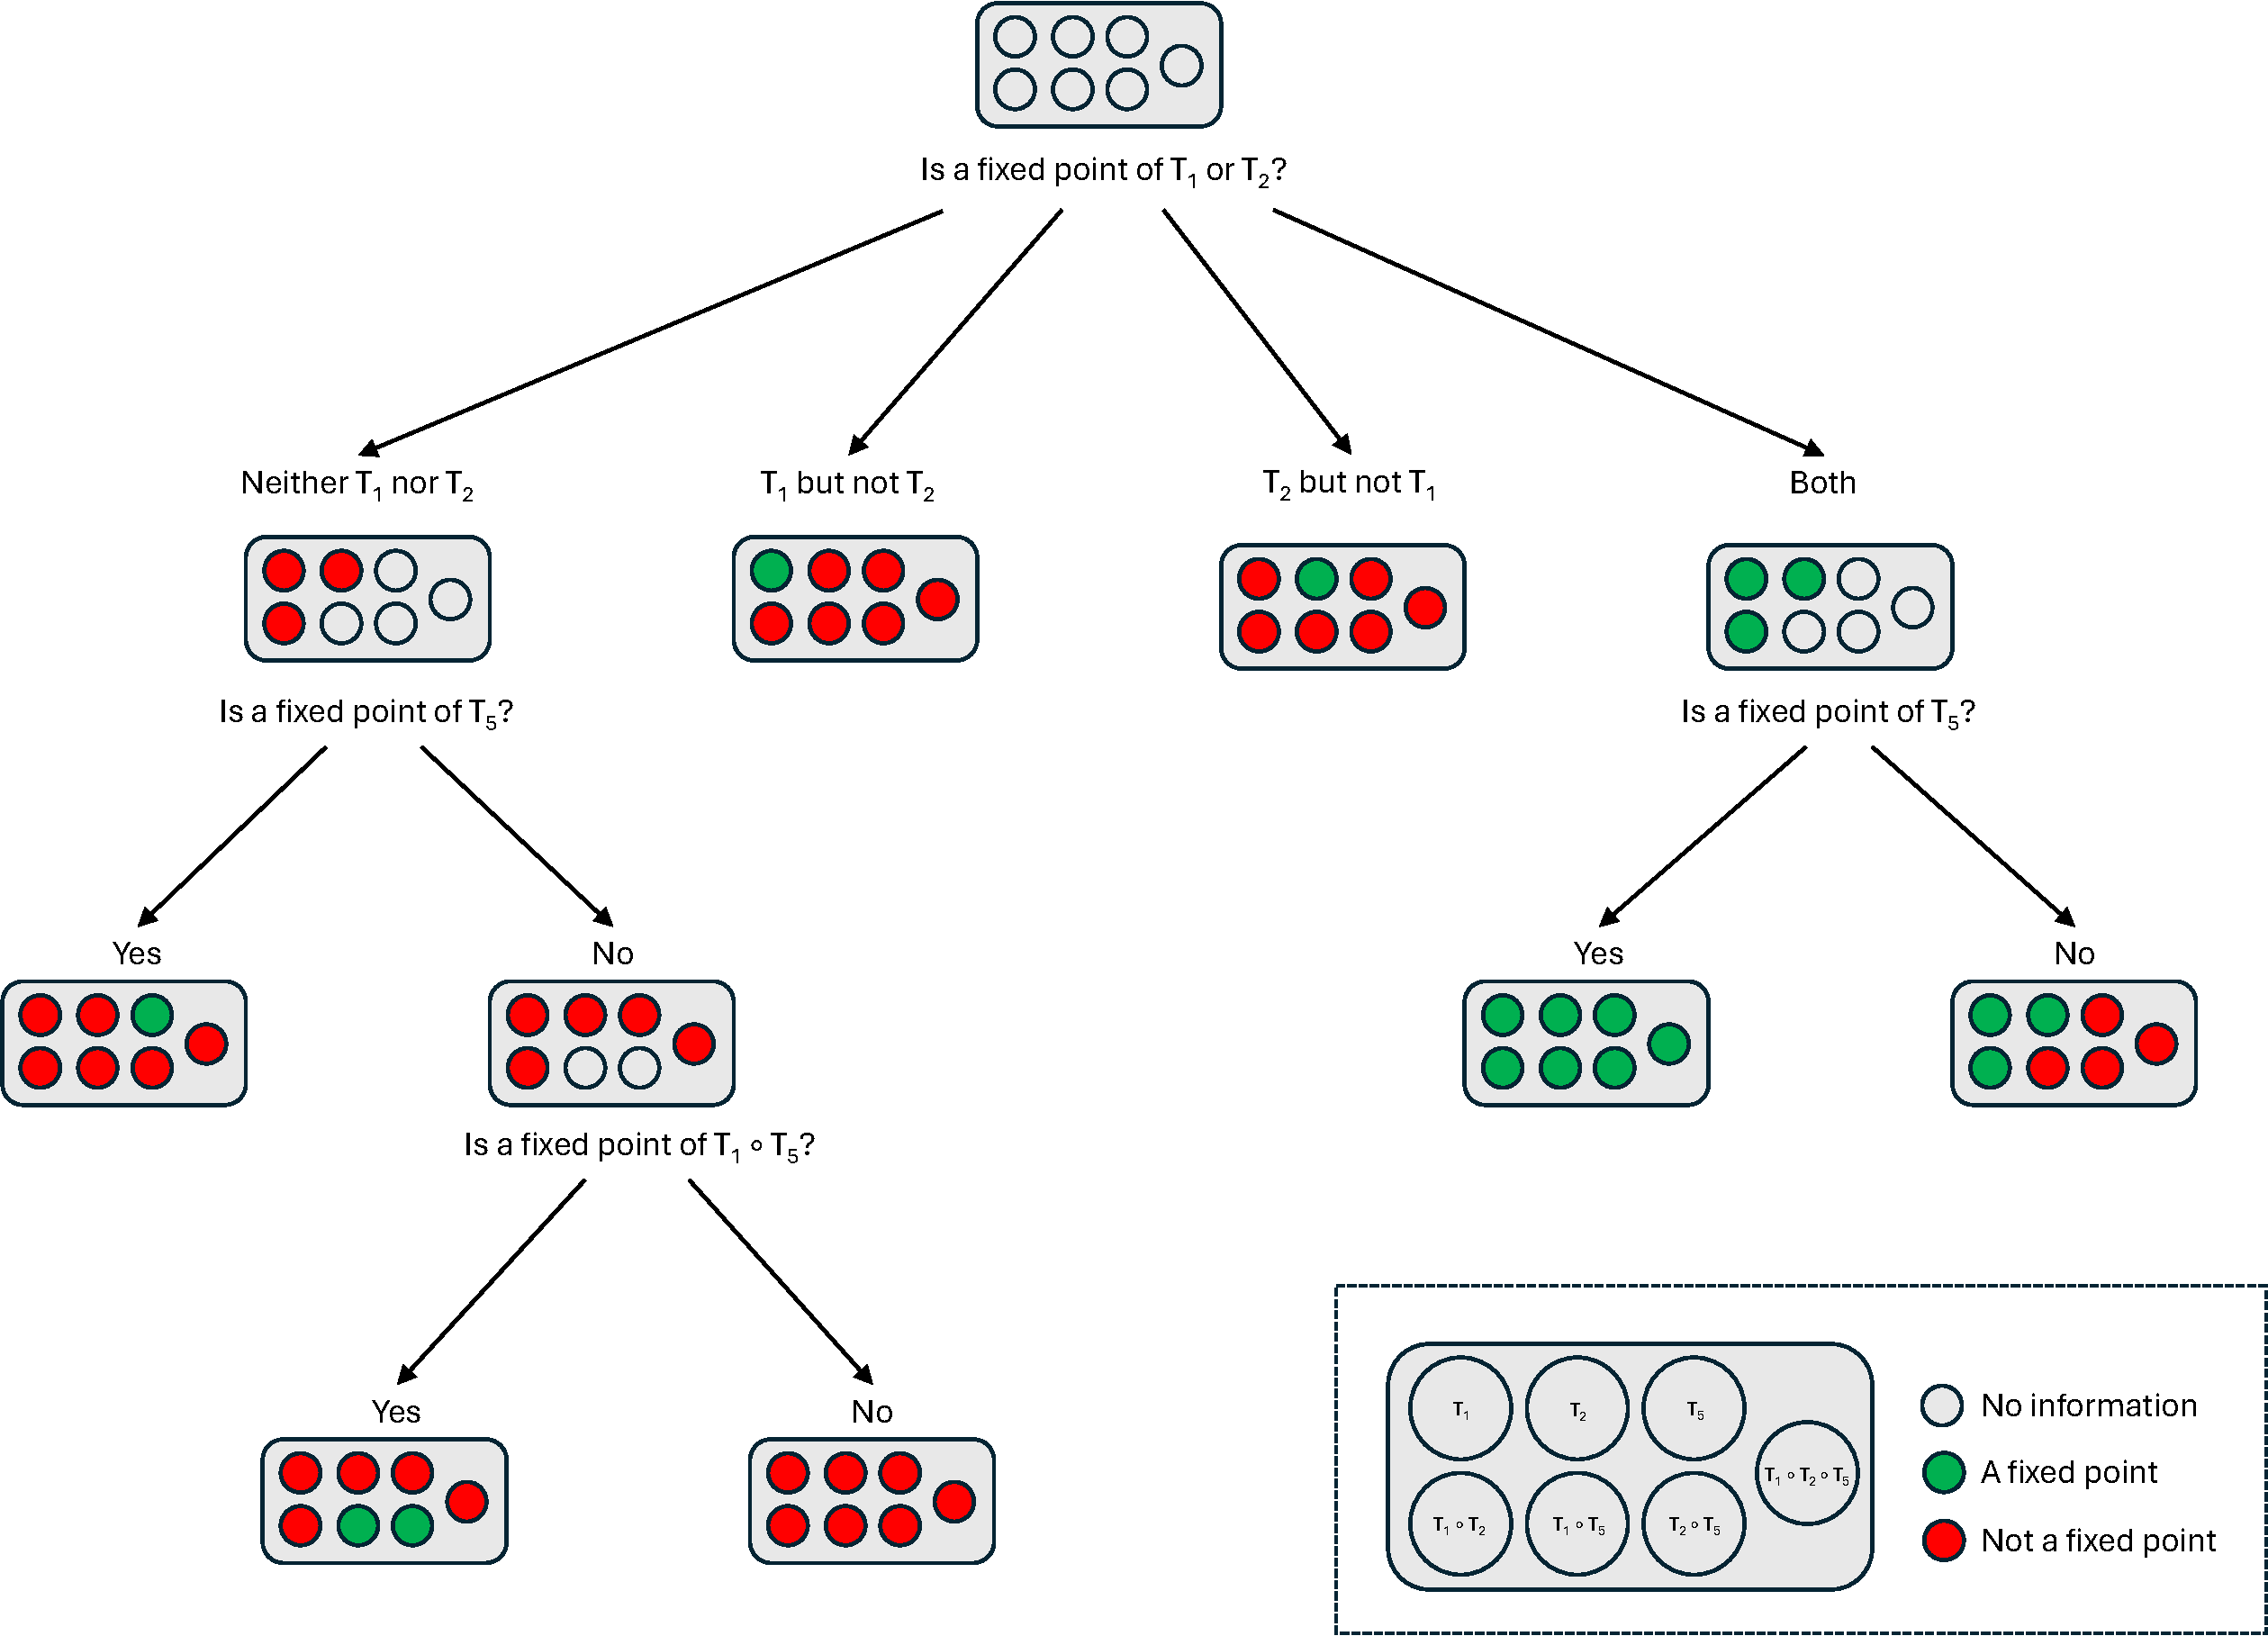
\includegraphics[width=\textwidth]{../images/fixed_point_decision_tree}
\caption{Decision tree to check if a state is a fixed point of a permutation
containing $T_1$, $T_2$, $T_5$, or compositions of their combinations.}
\label{fig:fixed_point_decision_tree}
\end{figure}



\begin{tcolorbox}[colback=orange!5!white,colframe=orange!75!black,title=TODO]
Enumerate combinatorially how many valid representative MDP states-action pairs
exist.
\end{tcolorbox}


\subsection{Rewards}
The reward received for transitioning from state $s_1$ to state $s_2$ given
action $a$ was taken, $R(s_1, s_2, a)$, consists of four components:

\begin{equation}\label{eqn:reward}
\text{R}(s_1, s_2, a) = -(C(s_1) + P(s_1, \theta))t_{s_1, s_2} - \Psi(a)
\end{equation}

Where

\begin{itemize}
    \item $t_{s_1, s_2}$ is the time spent in state $s_1$ before transitioning
    to state $s_2$;

    \item $C(s_1)$ is the instantaneous staffing cost, corresponding to the
    number of staff required to care for the patients per time unit.
    This can be calculated from the ward-state component of $s_1$, given by
    Equation~\ref{eqn:staffing_cost}.

    \item $P(s_1, \theta)$ is the instantaneous penalty, measured in staff per
    time unit, corresponding to a Stage 3-I patient not being in an isolation
    unit.
    This can be calculated from the ward-state component of $s_1$, given by
    Equation~\ref{eqn:penalty_cost}, where $\theta$ is some penalty parameter.

    \item $\Psi(a)$ is the cost of taking action $a$, corresponding to either
    an intra-ward move for patients of type $p$ (cost $\sigma_p$), an inter-ward
    move for patients of type $p$ (cost $\phi_p$), or moving a Stage 2 patient
    to surge (cost $\xi$).
    This is given by Equation~\ref{eqn:move_cost}.
\end{itemize}


\begin{align}
C &= G(M) + \sum_{i=1}^{2} \sum_{j=0}^{16} M_{i,j} \label{eqn:staffing_cost} \\[4mm]
P(s_1) &= \theta \sum_{j=0}^{15} M_{2,j} \label{eqn:penalty_cost} \\[4mm]
\Psi(a) &= \begin{cases}
0 \text{ if } b = d \\
\sigma_p \; \text{ if } b \text{ in the same ward as } d \\
\phi_p \; \text{ if } b \text{ in a different ward to } d \\
\xi \; \text{ if } d = 16
\end{cases} \label{eqn:move_cost}
\end{align}

where $s_1 = (M, p)$, $a = (b, d)$, and $G(M)$ represents a function that finds
the minimum number of nurses required to cover the Stage 2 patients, when pairs
of adjacent patients can be seen by the same nurse, as shown in
Figure~\ref{fig:resource_use}.


\subsection{Simulation Model}
The simulation model is parametrised as described in
Section~\ref{sec:description}.
Additionally we parametrise the isolation penalty with $\theta=8$.


\section{Reinforcement Learning Framework}\label{sec:rlframework}
Reinforcement learning is a model-free unsupervised learning that allows a
central agent to learn optimal policies as it explores the state space during a
simulation run.
One standard algorithm is Q-learning, with overviews given in
\cite{suttonbarto1998} and \cite{watkins1992}.
The idea is that each MDP state and action pair, $(s, a)$ with $s \in S$ and
$a \in A_s$, has some value $Q(s, a)$, called $Q$-values, representing the
expected long term reward for taking action $a$ when in state $s$, and
following an optimal policy from then on.
An optimal policy is, for each state, the action that gives the maximum
expected reward, given by Equation~\ref{eqn:optimal_policy}.

 \begin{equation}\label{eqn:optimal_policy}
 a^{\star} = \arg\!\max_{a \in A_s} Q(s, a)
 \end{equation}

The $Q$-values are found by iteratively updating them, as the simulation visits
states, performs actions, and observes some reward, until convergence.
The update, implemented once state $s'$ has been reached, after taking action
$a$ in state $s$, and observing a reward $R(s, s', a)$ is given in
Equation~\ref{eqn:q_update}.

\begin{equation}\label{eqn:q_update}
Q(s, a) \leftarrow (1 - \alpha) Q(s, a) + \alpha \left(R(s, s', a) + \gamma \max_{a' \in A_s'} Q(s', a') \right)
\end{equation}

Here $\alpha \in (0, 1]$ is the learning rate, a parameter that indicates how
important new information is, or how quick the agent is to trust new
information; and $\gamma \in [0, 1)$ is the discount factor, a parameter that
indicates how important future rewards are as opposed to immediate rewards.
The ICU ward is stochastic, and so we anticipate a medium to low learning rate
$\alpha$ would be required to overcome the variability in the rewards.
The aim is for a general state of high reward throughout the ICU's operating
times, and so future rewards are just as important as immediate rewards, so we
anticipate a high discount factor $\gamma$ would be beneficial.
In particular, as the rewards are dependent on the time between updates
(Equation~\ref{eqn:reward}), immediate rewards are far less meaningful than long
run average rewards - for example, one long interval with low instantaneous
reward may look better than many shorter periods of high rewards, but it is the
long run average that matters.

The reinforcement learning framework used is developed in Python.
Due to the very high number of possible states-action pairs, the framework
utilises high performance libraries such as Numpy~\cite{numpy20} and
Numba~\cite{numba15}, and was optimised for both speed and memory with help from
conversations with Google Gemini~\cite{googlegemini26} to learn and steer some
of the software development.
It is fully unit-tested and verified, and openly available
at \url{https://github.com/geraintpalmer/bed_moves_policy}.

The $Q$-values are stored in a Numba typed dictionary, an implementation of a
hash table, that maps state-action pairs to Q-values, which are generally kept
in memory.
At the beginning of a run, all state-action pairs are unexplored, and the
$Q$-value dictionary is empty.
When state-action pairs are visited for the first time, the state-action pair is
added to the dictionary, mapping it to the $Q$-value calculated using
Equation~\ref{eqn:q_update}, however this may require the $Q$-value of other
unexplored state-action pairs.
In these cases, we want the baseline $Q$-value for unexplored states to be
undesireable.
Assuming $Q$-values follow a Normal distribution, we use their 20th percentile
as a default value, $Q_{0.2}$, using Equation~\ref{eqn:averageQ}, which can be
obtained by keeping track of the running mean and variance of the rewards,
$\bar{R}$ and $s_R^2$, using updates such as Welford's update \cite{welford62},
and the 20th percentile of the standard Normal distribution, $z_{0.2}$.

\begin{equation}\label{eqn:averageQ}
Q_{0.2} = \frac{\bar{R} - z_{0.2} s_R^2}{1 - \gamma}
\end{equation}


\subsection{State Hashing}\label{sec:hashing}
Due to the vast number of potential state-action pairs, storing full tuples and
matrices in the Q-table is very memory intensive.
Therefore in order to preserve memory, we define a reversible hash between
state-action pairs $(s, a) = ((M, p), a)$ and 64-bit integers (from
$-2^{63}$ to $2^{63} - 1$), that is a 19-digit integer.

We do this with the follow form of mixed radix encoding, given by
Equation~\ref{eqn:hashing}, where $\langle A, B \rangle_F = Tr(A^T B)$ is the
Frobenius inner product~\cite{calderolver25}, and the matrix $W$ is given in
Equation~\ref{eqn:hash_weights}.

\begin{equation}\label{eqn:hashing}
H((M, p), (b, d))) = 100000\langle M, W \rangle_F + 10000p + 100b + d
\end{equation}

\begin{equation}\label{eqn:hash_weights}
W = \begin{pmatrix}
3 \times 19 \times 4^{14} & 2 \times 19 \times 4^{14} & 1 \times 19 \times 4^{14} \\
3 \times 19 \times 4^{13} & 2 \times 19 \times 4^{13} & 1 \times 19 \times 4^{13} \\
3 \times 19 \times 4^{12} & 2 \times 19 \times 4^{12} & 1 \times 19 \times 4^{12} \\
3 \times 19 \times 4^{11} & 2 \times 19 \times 4^{11} & 1 \times 19 \times 4^{11} \\
3 \times 19 \times 4^{10} & 2 \times 19 \times 4^{10} & 1 \times 19 \times 4^{10} \\
3 \times 19 \times 4^9 & 2 \times 19 \times 4^9 & 1 \times 19 \times 4^9 \\
3 \times 19 \times 4^8 & 2 \times 19 \times 4^8 & 1 \times 19 \times 4^8 \\
3 \times 19 \times 4^7 & 2 \times 19 \times 4^7 & 1 \times 19 \times 4^7 \\
3 \times 19 \times 4^6 & 2 \times 19 \times 4^6 & 1 \times 19 \times 4^6 \\
3 \times 19 \times 4^5 & 2 \times 19 \times 4^5 & 1 \times 19 \times 4^5 \\
3 \times 19 \times 4^4 & 2 \times 19 \times 4^4 & 1 \times 19 \times 4^4 \\
3 \times 19 \times 4^3 & 2 \times 19 \times 4^3 & 1 \times 19 \times 4^3 \\
3 \times 19 \times 4^2 & 2 \times 19 \times 4^2 & 1 \times 19 \times 4^2 \\
3 \times 19 \times 4^1 & 2 \times 19 \times 4^1 & 1 \times 19 \times 4^1 \\
3 \times 19 & 2 \times 19 & 1 \times 19 \\
9 & 3 & 1
\end{pmatrix}^T
\end{equation}

The first 15 columns use a counting scheme in base 4, as there are only 4
configurations for each of these columns.
Now consider the 15th column, the entries are integers in $\{0, 1, 2\}$, and so
the elements of this column can be counted in base 3.
Noting however, due to the constraint that the sum of this column cannot exceed
2, that the maximum value of this column would be 18, corresponding to
$\left(\begin{smallmatrix}2\\0\\0\\\end{smallmatrix}\right)$, then we can use
base 18 to count this entire column.
Together then, $M$ can be represented by by numbers between 0 and 20401094655,
that is by at most an 11 digit number.
Now using positional concatenation (base 10) we can including the arriving
patient type $p$ and action $a = (b, d)$ gives us a 16 digit
number, well within the confines of 64-bit integers.

As an example $H((M^{\star}, 2, (11, 4)) = 2025762603821104$, where $M^{\star}$
is the ward state given in Equation~\ref{eqn:example_M}.


\subsubsection{Choosing Representative States and Actions}\label{sec:representative}
In Sections~\ref{sec:state_equivalences} and~\ref{sec:action_equivalences} we
introduced the idea of representative ward states and representative action,
that can stand in place for all ward states and all actions in the same
equivalence class.
During the simulation run, whenever the algorithm encounters a state, the
algorithm will update the Q-value for its equivalent representative state,
ensuring faster learning and a smaller exploration space.

The representative states for a particular equivalence class are chosen as
those states with the smallest hash.
Similarly for actions.

Practically, this means that whenever the simulation reaches state $M$, then
the hash for all states in $[M]$ are found, and the minimum is chosen.
Similarly for actions.


\subsection{Training Framework}
During the simulation's training run, actions are selected using the
$\epsilon$-greedy policy \cite{suttonbarto1998}, that is, for some probability
$\epsilon \in [0, 1]$, the agent will choose the best discovered action so far,
using Equation~\ref{eqn:optimal_policy}, with probability $\epsilon$, and
choose a random action with probability $1 - \epsilon$.
That is, the agent \textit{explores} with probability $1 - \epsilon$, and
\textit{exploits} with probability $\epsilon$.

Exploration versus exploitation is an important concept in reinforcement
learning, especially in such vast state-spaces.
Exploration, or a low $\epsilon$, is important to be able to discover new
state-action pairs, however spending too much time exploring can be detrimental,
as it wastes time and resources on discovering states that would be seldom
visited when following the optimal policy.
Exploitation, or a high $\epsilon$, ensures that relevant states are revisited
many times, helping to gain enough information on these state-action pairs that
their $Q$-values are updated enough times for these to be a good approximation
of the expected future rewards.
We choose to begin the training run with a low $\epsilon$ and gradually increase
is throughout the run - exploring early to find plausible optimal policies, and
exploiting later to refine them.

With such a vast state space, and high stochasticity, convergence for all states
is practically impossible, and we must settle on very long enough run times to
obtain good-enough $Q$-values to read off optimal policies.
These long run times are still computationally expensive and time intensive.
We therefore train the agent in a parallel framework, visualised in
Figure~\ref{fig:training_framework}.


\begin{figure}
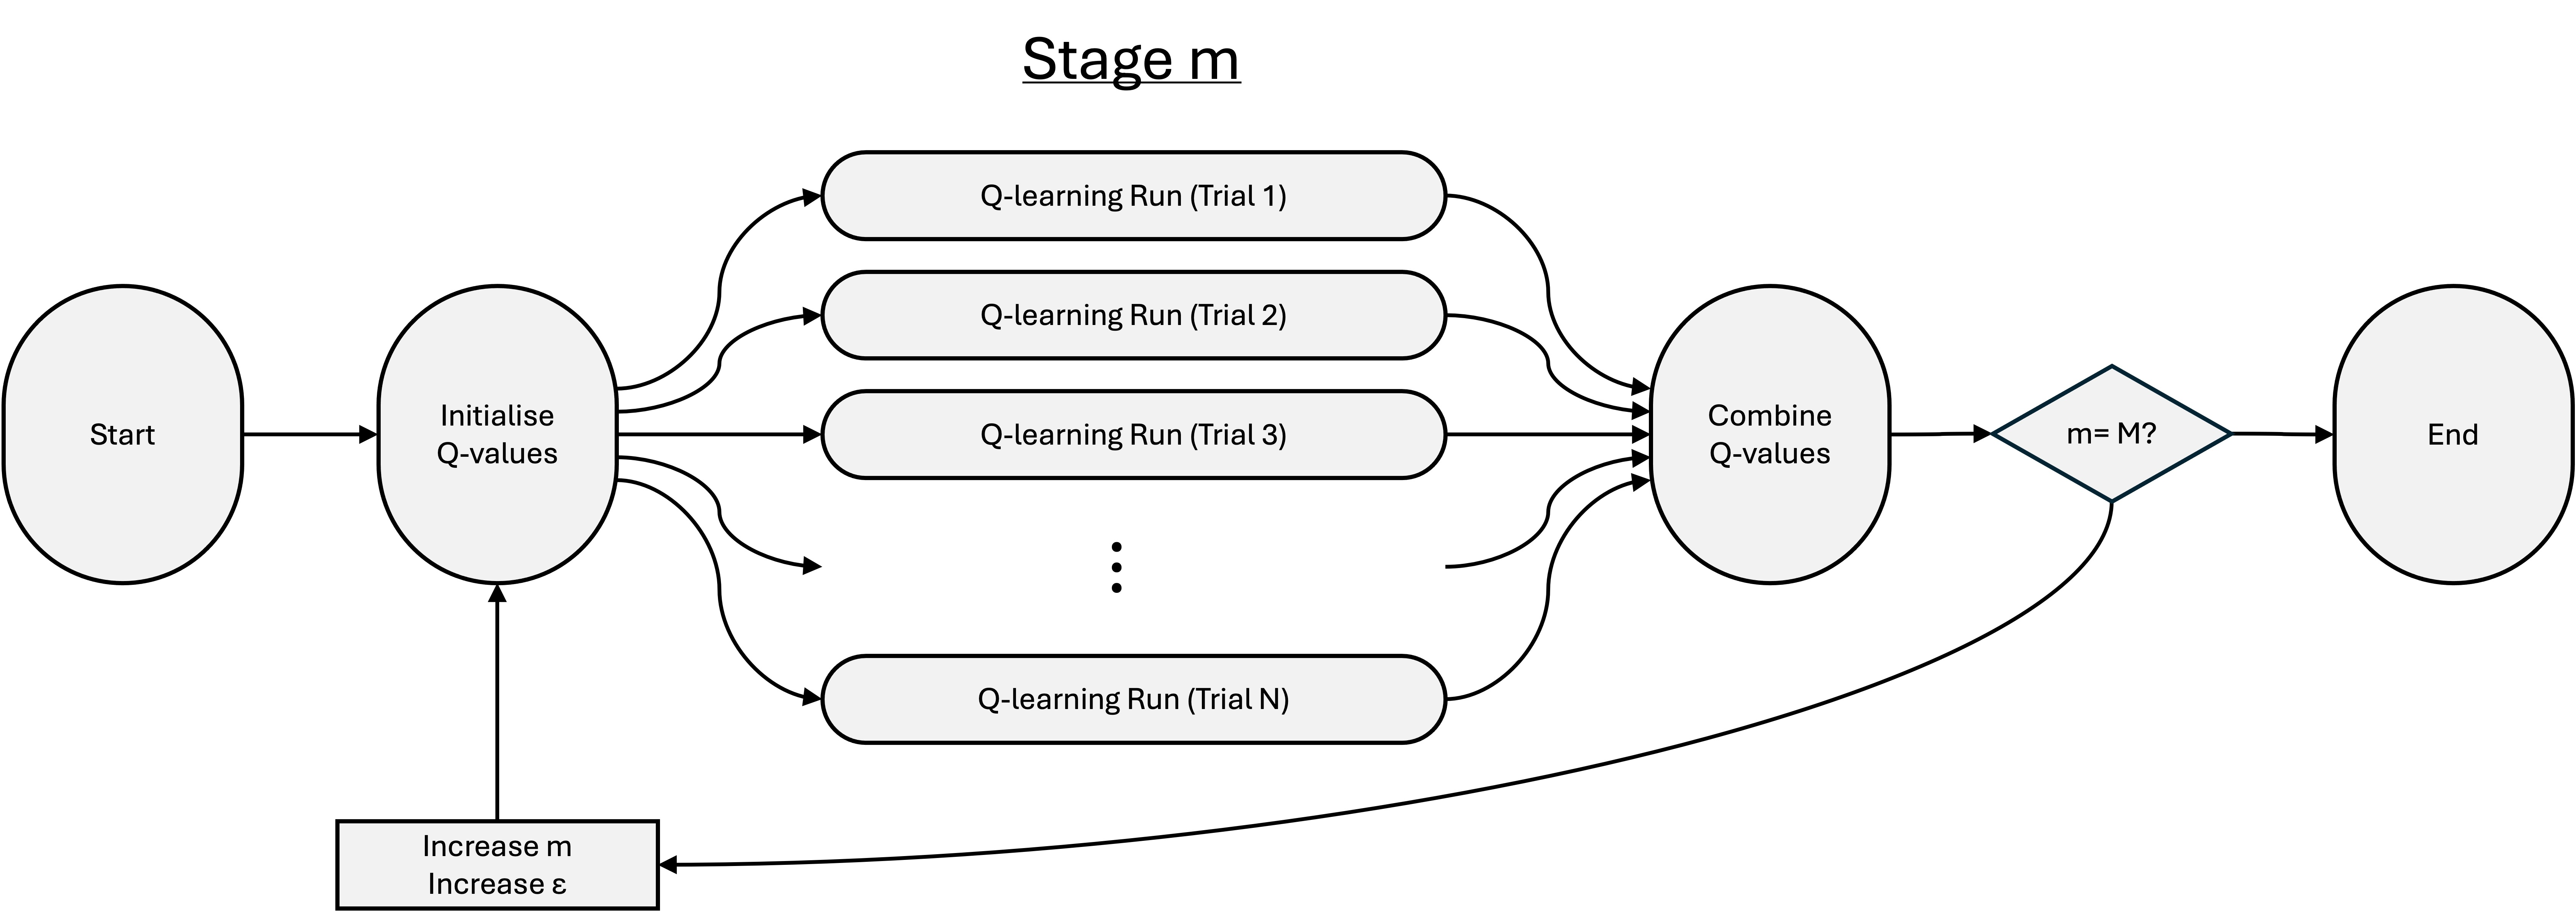
\includegraphics[width=\textwidth]{../images/qlearning_setup}
\caption{Framework used for training the model.}
\label{fig:training_framework}
\end{figure}

We train the model over $M$ stages, utilising $N$ parallel workers.
At stage $m=0$, $Q$-value tables are initialised as empty, that is no
states-action pairs have been discovered yet, and we set $\epsilon = 0$ for full
exploration.
These $Q$-value tables are replicated $N$ times, and split over $N$ parallel
workers, each running its own training simulation, updating its own table of
$Q$-values for a particular stretch of time.
Once these parallel training runs are complete, each worker will have its own
distinct table of $Q$-values: let $Q_n(s, a)$ represent the $n^{\text{th}}$
worker's estimate of the $Q$-value for the $(s, a)$ state-action pair.
Workers also keep track of the number of visits to each state-action pair, let
$h_n(s, a)$ be the number of times worker $n$ visited that state-action pair.
These tables are then combined, weighting each $Q$-value by the number of
visits, that is:

\begin{equation}
Q(s, a) = \frac{\sum_{n=0}^N Q_n(s, a) h_n(s, a)}{\sum_{n=0}^N h_n(s, a)}
\end{equation}

In the next state, we update $\epsilon \leftarrow \epsilon + \sfrac{1}{M}$,
gradually increasing the agents rate of exploitation.
Then $Q$-values are initialised with the combined $Q$-value tables found at the
end of the last stage, the $h_n$ are reset to zero, and the training is repeated
on parallel workers.
This ensures that at the first stage we have full exploration, and by the final
stage we have full exploitation, with $\epsilon$ increasing linearly over the
stages.

After each stage the combined $Q$-values are saved and so the incumbent policy
can be evaluated by running the simulation, without any $Q$-learning, choosing
actions based on that incumbent policy.

As it is standard for any run of a simulation to begin from an empty state, a
larger number of parallel trials at each stage yield the added benefit of
obliging the agent to sufficiently explore early, near-empty states; despite
visits to these states possibly being rarer in reality.
This can be beneficial because the agent needs to learn a route from an empty
state to the commonly visited states, especially those visited under an optimal
policy, to ensure that any time a simulation is run it quickly reaches useful
states.
This is vital when researting each stage, but also for policy evaluation.


\subsection{Pruning}
As the number of theoretically possible state-action pairs is so large, the
memory constraints of a computer makes running the algorithm difficult in
practice, as the $Q$-value table grows with exploration.
However, the practically reachable space of state-action pairs, when following
an optimal, or even just a reasonable, policy, is much smaller.
This is often called the `on-policy distribution' \cite{suttonbarto1998}.
Therefore any state-action pairs in the suboptimal trajectory space, that is
those not in the on-policy distribution, can generally be ignored, reducing the
$Q$-value table and saving memory.

After the end of each stage, these states are identified as those who have not
been visited frequently, if at all, and so can be pruned.
We prune all state-action pairs whose number of hits $h_n(s, a)$ is less than
some chosen limit $\tilde{h}$.
This not only helps save memory, but also cleans the data: the simulation is
highly stochastic, and for states with $h_n(s, a) < \tilde{h}$, its $Q$-value
will have been based on $h_n(s, a)$ observations only, meaning that for very
small $\tilde{h}$ this is just stochastic noise and so cannot meaningfully
estimate the expected rewards.

Note that due to the way in which $Q$-values are passed from stage to stage, it
is possible to reach the end of a stage and for a particular state-action pair
to be present in the table but have been visited zero times: for example if a
pair was visited in stage $n-1$, it was passed to stage $n$ and its number of
hits reset to zero, but then not visited at all in stage $n$.
This would be a good candidate to prune and so not pass to stage $n+1$.




\section{Experiments}
For a particular run, we evaluate each stage' incumbent policy by running the
simulation for 60 trials, for a 30,000 time units, and a warm-up time of 5,000
time units, and recording the overall cost running the ICU for the remaining
25,000 time units when exploiting that incumbent policy.
An initial `random` policy is evaluated for comparison.

First we train the agent using the framework described in
Section~\ref{sec:rlframework}, choosing $\alpha = 0.6$ and $\gamma = 0.6$.
During training each stage was run for 500,000 time units, using 20 parallel
workers per stage.
Figure~\ref{fig:base_run} shows these results.
We see that as the stages increase (and hence more training), the agent makes
very quick gains in the early stages as the agent explores more, and then slower
gains as the agent exploits and refines the policies it has already learned.
In this case the agent has made gains from a cost of 366681.25 using the random
policy, to 273569.88 using the policy at the end of the 21 stages, an
improvement of 25.4\%.

\begin{figure}
\begin{center}
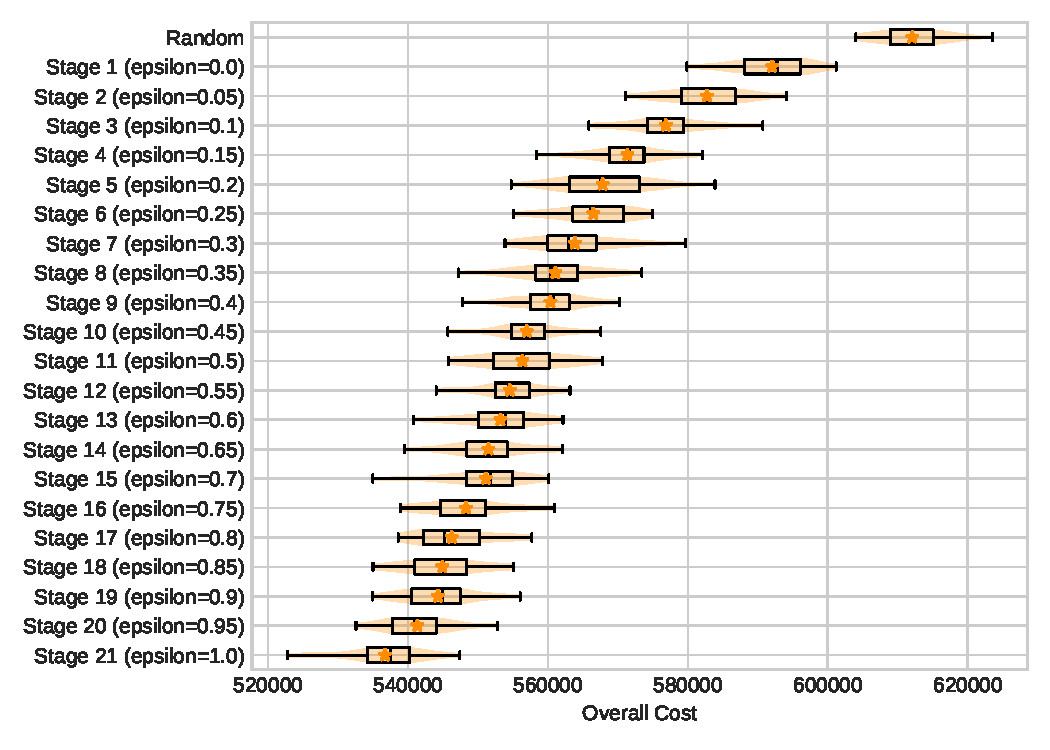
\includegraphics[width=0.85\textwidth]{../src/experiments/test_run/results/cost_by_stage}
\end{center}
\caption{Evaluation of the incumbent policies across the stages.}
\label{fig:base_run}
\end{figure}

As there is such a huge amount of state-action pairs, it is practically
impossible to estimate whether the policy has converged or not, though we see
any improvements in cost slowing down as the stages increase.
We can also count the number of unique state-action pairs visited per stage
during the training process, shown in Figure~\ref{fig:base_run_visited}.
We see some tapering-off of the number of new states-action pairs visited,
indicating both a decreasing tendency to explore (from the increasing
$\epsilon$), and a gradual saturation of states from previous explorations.

\begin{figure}
\begin{center}
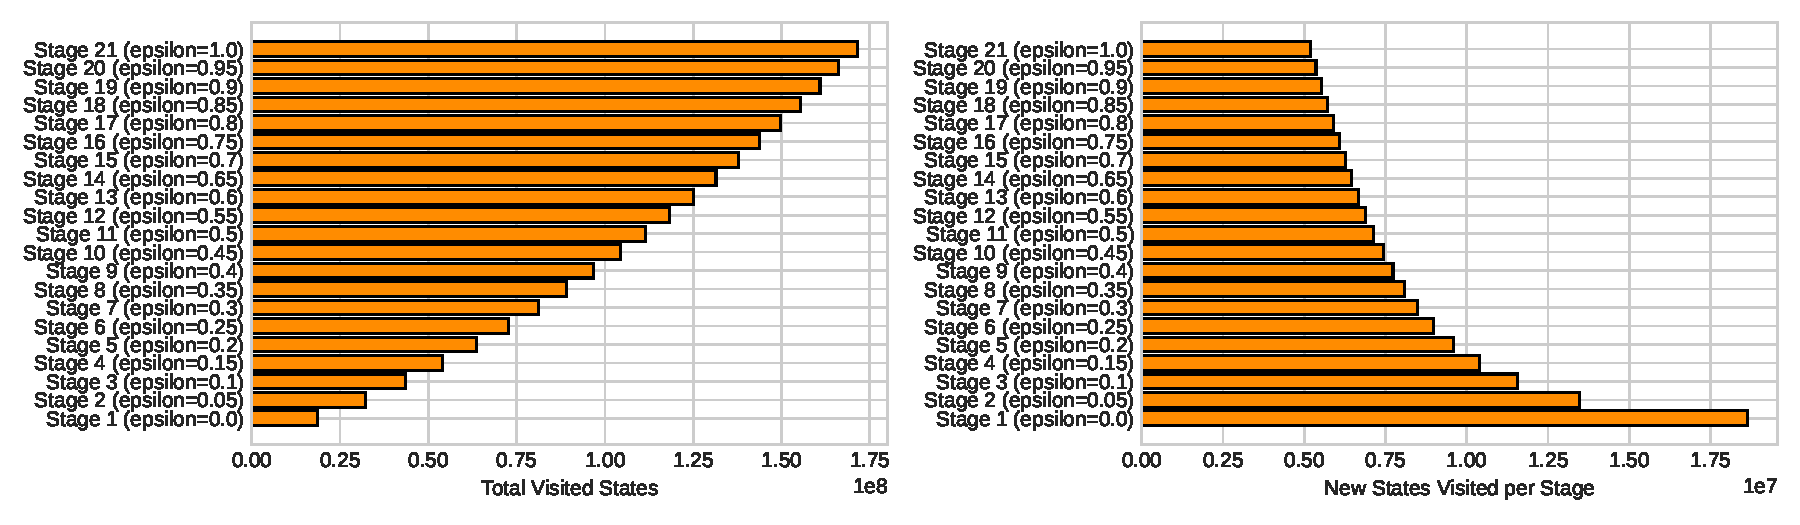
\includegraphics[width=0.95\textwidth]{../src/experiments/test_run/results/unique_visits_per_stage}
\end{center}
\caption{Number of state-action pairs visited in each stage of the training
process.}
\label{fig:base_run_visited}
\end{figure}


\subsection{Effect of the learning rate $\alpha$}
Using this setup then, we can also look at the effect of the learning rate
$\alpha$.
Figure~\ref{fig:vary_alpha} shows the percentage improvement in using the
incumbent policy per stage for different values of $\alpha$ (left), and the
percentage improvement after all 21 stages for different values of $\alpha$
(right).

\begin{figure}
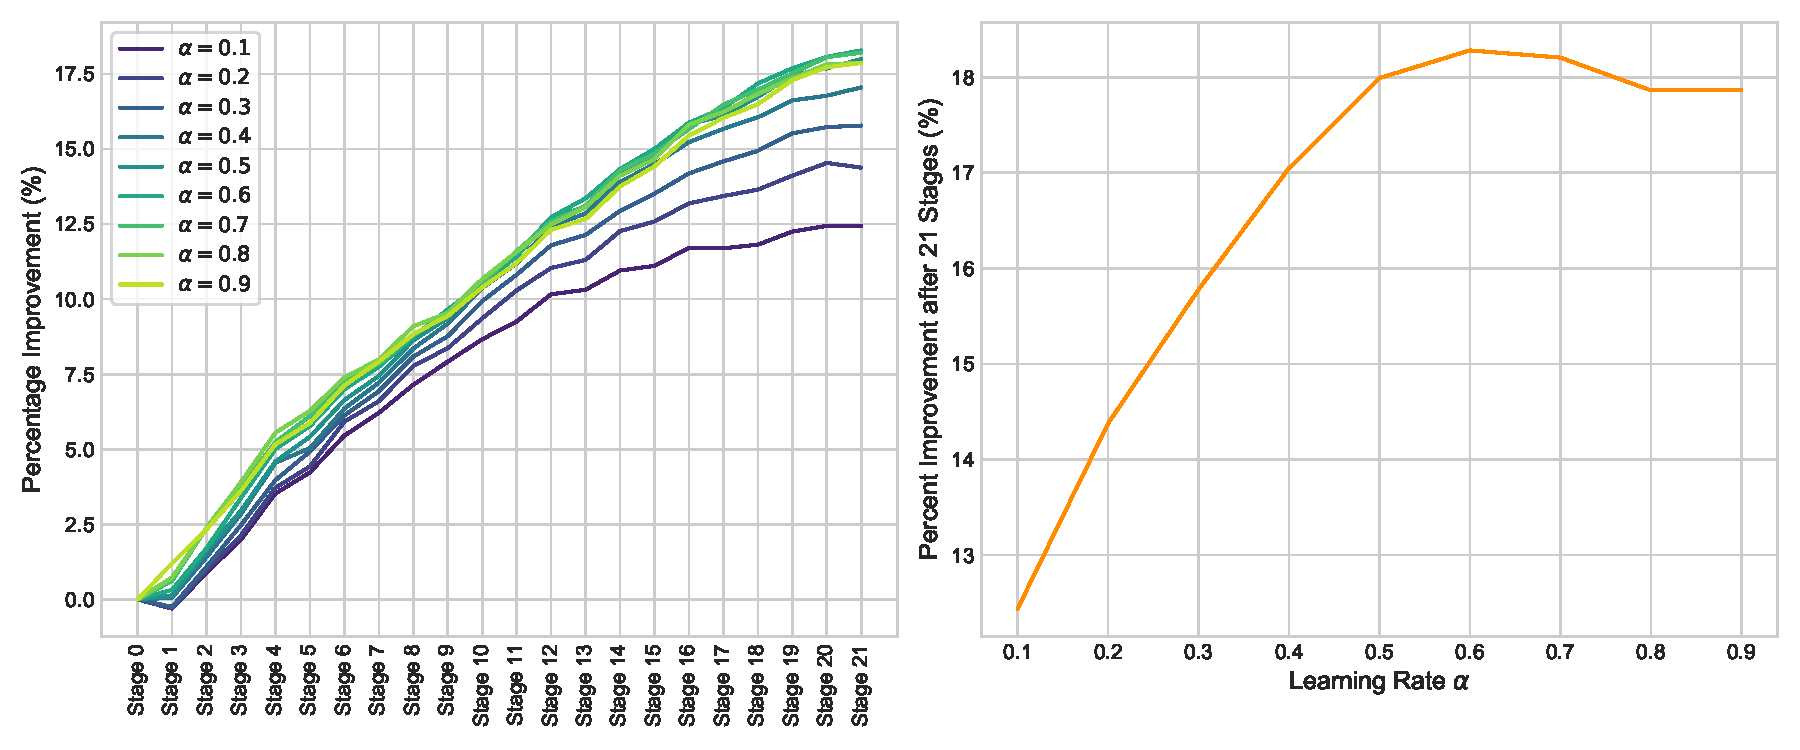
\includegraphics[width=\textwidth]{../src/experiments/vary_alpha/vary_alpha}
\caption{The effect of varying the learning rate $\alpha$.}
\label{fig:vary_alpha}
\end{figure}

We immediately see from the left plot that the improvement peaks when
$\alpha=0.6$, indicating that this is the ideal learning rate for this problem,
when running under the current setup.
However the right plot shows the agent's behaviour as the training progresses:
a smaller learning rate results in slower learning (a less steep curve); a high
learning rate has faster learning, but cannot smooth out stochasticity of
rewards as effectively; while a moderate learning rate can learn quickly and smooth
out variability.
The speed of learning is important in our case is important: as it would be
impractical to run the algorithm until convergence we have to choose some
temporal cut-off, and so we want as much learning to occur in the time allotted
as possible.


\subsection{Effect of the discount factor $\gamma$}
We can also look at the effect of the discount factor $\gamma$.
Figure~\ref{fig:vary_gamma} shows the percentage improvement in using the
incumbent policy per stage for different values of $\gamma$ (left), and the
percentage improvement after all 21 stages for different values of $\gamma$
(right).

\begin{figure}
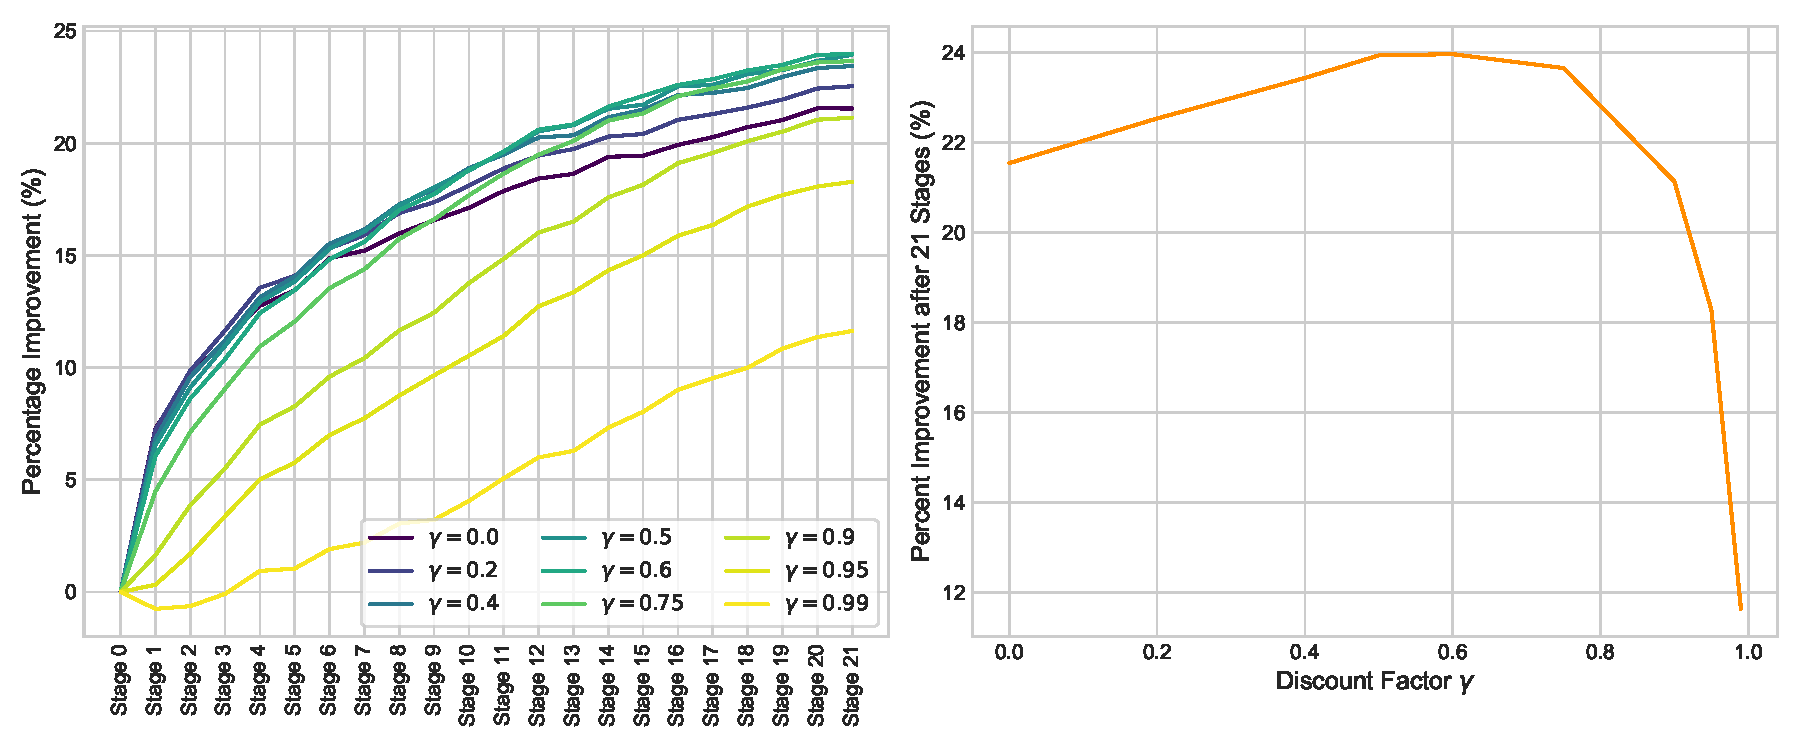
\includegraphics[width=\textwidth]{../src/experiments/vary_gamma/vary_gamma}
\caption{The effect of varying the discount factor $\gamma$.}
\label{fig:vary_gamma}
\end{figure}

Again we can immediately see from the plot on the left that the improvement
peaks when $\gamma$ is around 0.5-0.6.
Considering the right plot which shows the agent's behaviour as the training
progresses: a high discount factor results in slower learning (a less steep
curve), this is due to each update requiring a larger input from future rewards,
which themselves need to be well-learned; a small discount factor has faster
learning, but account for steady-state or average long-run rewards as
effectively.
Again, the speed of learning due to the need to choose some arbitrary
temporal cut-off.

\subsection{Effect of the traffic intensity}
Bed moves policies might have a greater impact on some ICU wards over other, or
there might be some situation where finding optimal bed moves policies can have
greater impact.
One feature that is likely to have an effect is the ward's business, or the
traffic intensity of the ward.
To test this, introduce some factor $m$, and multiply all arrival rates by $m$,
while keeping the service rates fixed.
In this way increasing $m$ increases the traffic intensity $\rho$ of the ward
linearly, due to summation of traffic intensities across customer classes:

\begin{equation}
\rho = \rho_{\text{green}} + \rho_{\text{amber}} + \rho_{\text{red}} =
\frac{m}{17}\left(
\frac{\lambda_{\text{green}}}{\mu_{\text{green}}} +
\frac{\lambda_{\text{amber}}}{\mu_{\text{amber}}} +
\frac{\lambda_{\text{red}}}{\mu_{\text{red}}}
\right)
\end{equation}

To keep costs and training epochs relatively comparable, we reduce the maximum
training and evaluation times by a factor $m$ also.
Figure~\ref{fig:vary_rho} shows the overall evaluation cost, ad $\rho$ varies,
for each stage of training.

\begin{figure}
\begin{center}
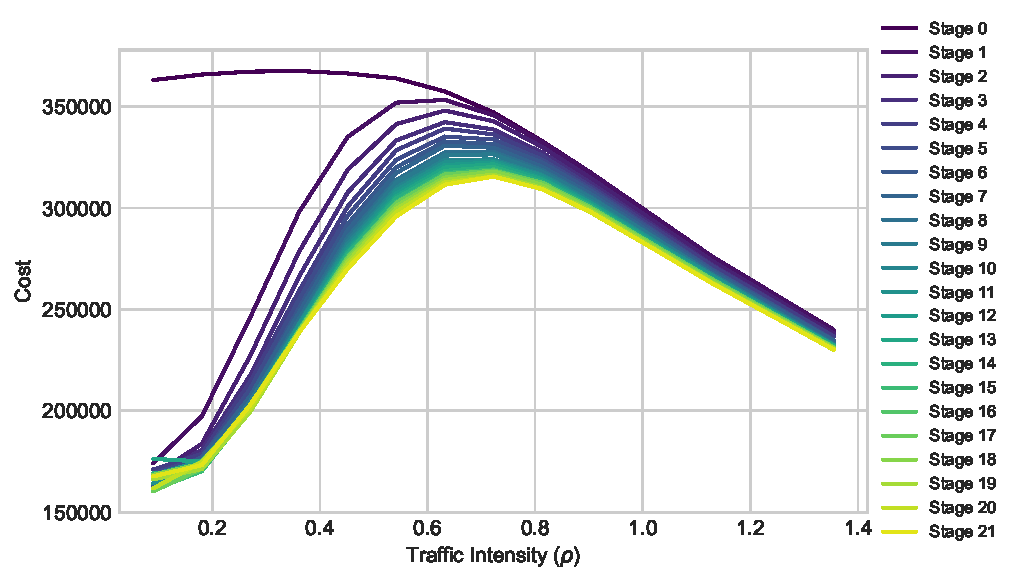
\includegraphics[width=0.6\textwidth]{../src/experiments/vary_arrivals/vary_arrivals}
\end{center}
\caption{The effect of varying the traffic intensity, $\rho$.}
\label{fig:vary_rho}
\end{figure}

When $\rho$ is small, we see that there are huge gains to be made, and that most
of these gains happen in the early stages, that is after not much training.
This implies that these are easy or obvious changes that can be made using human
instinct, and a reinforcement learning algorithm may not be needed in practise.
The large gains may also show that in such an empty ward, it is easy to reach an
`ideal` scenario, where no penalties or extra staffing is required, as the near
empty system is not very complex.

When $\rho$ is very large, there is hardly any gains to be made.
This may be because ward is so busy that any bed move actions are not helpful,
and penalties and extra staffing are unavoidable whatever moves are taken.
Here there is not enough `wiggle room` to influence much.

This implies that the ideal times to invest in a bed moves policy is for
moderate traffic intensities, where $0.3 < \rho < 0.6$. Here large to moderate
gains are still possible, however these gains occur in the later stages of
training, implying they are less obvious and hence the power of the
reinforcement learning algorithm is useful. This is a sweet spot where there is
sufficient complexity in the system to require a policy, and enough `wiggle
room` to make substantial gains.


\section{Human-Readable Policies}
\begin{tcolorbox}[colback=orange!5!white,colframe=orange!75!black,title=TODO]
Idea: Currently the policies that come from the reinforcement learning is a
mapping from millions / tens of millions of states to optimal actions. I wonder
if we can use some sort of machine learning / clustering algorithm to simplify
this into general human-readable `guidelines` rather than a full detailed
policy. This simplified policy would of course be less effective than the full
policy, but this is something that can be measured and analysed.
\end{tcolorbox}

\bibliographystyle{plain}
\bibliography{refs}

\end{document}